\chapter[Model-based Reconstruction for Real-Time Phase-Contrast Flow MRI]
{Model-based Reconstruction \\ 
for Real-Time Phase-Contrast Flow MRI}
\chaptermark{Model-based Phase-Contrast Flow MRI} \label{Chp:mir-pc}

A novel mathematical model of phase-contrast flow MRI is developed based on the assumption that the flow-compensated and flow-encoded images have the same magnitude, but only differ in phases. This assumption is especially true in real-time phase-contrast flow MRI at high temporal resolutions and in conditions where laminar flows are measured. The unknowns (magnitude image, phase-contrast map, and one set of coil sensitivity maps) in this model can be jointly estimated by \acs{IRGNM}. This method avoids the phase-difference calculation and directly applies regularizations on the phase-difference map, which substantially reduces random phase noise.

\section{Introduction}
Based on the physical relationship between a gradient-induced phase shift and the velocity of spins in a corresponding NMR \cite{1960_PC_Hahn} or MRI experiment \cite{1982_PC_Moran} as well as initiated by early seminal applications \cite{1984_PC_Bryant,1984_PC_Dijk,1991_PC_Pelc}, there is nowadays extensive clinical use of velocity-encoded phase-contrast techniques for quantitative MRI studies of blood flow. For relevant reviews see \cite{2005_PC_Gatehouse,2009_PC_Srichai}. More recently, technical advances in real-time MRI \cite{2010_20ms_Uecker}, which rely on regularized NLINV reconstructions of highly undersampled radial gradient-echo acquisitions \cite{2008_NLINV,2010_NLINV_Heart,2012_Schaetz,2014_Temp_Fidelity}, have been extended to cardiovascular applications \cite{2010_RTCMR_Zhang,2013_SSFP_Voit,2014_RT_Zhang} and, in particular, to phase-contrast flow MRI \cite{2012_PC_Joseph,2014_PC_Joseph,2015_PC_Asym}. These and other accelerated flow MRI studies \cite{2005_PC_ktSENSE,2012_PC_Kim} combine parallel imaging with a phase-difference computation \cite{2004_MRI_Bernstein} of two complex images with complementary velocity encodings, i.e., a flow-compensated and a flow-encoded acquisition. As a consequence, phase-difference maps present with extensive phase noise in areas of low or no MRI signal (e.g.~air). Although tolerable in many cases, the presence of strong noise may complicate the definition of the true vessel lumen and therefore affect quantitative flow analyses, hamper the assessment of flow in small vessels or, in case of radial undersampling, enhance residual streaking artifacts. 

On the other hand, model-based approaches in MRI are a well-introduced concept for a variety of post-processing problems, i.e., image segmentation. However, less attention has been paid to model-based reconstructions, despite the fact that respective techniques have previously been detailed in an excellent review \cite{2010_MIR_Fessler}. While selected proposals deal with accelerated $T_2$ mapping \cite{2009_MIR-T2_Block,2011_T2_Sumpf,2014_T2_Sumpf}, fat-water imaging \cite{2004_IDEAL}, inhomogeneity-corrected $T_2^*$ mapping \cite{2009_fim_t2s_me_TMI}, quantitative susceptibility mapping \cite{2013_nlinv_QSM_MRM} and reconstructions of the diffusion tensor \cite{2015_mb_DTI_NBM}, preliminary attempts have also been made to use constrained reconstruction techniques for accelerated phase-contrast flow MRI \cite{2013_PC_CD_Kwak,2015_CD_Sun}. For example, Kwak et al.~\cite{2013_PC_CD_Kwak} reconstructed flow-compensated and flow-encoded images by regularizing the sparsity of the complex-difference image \cite{2004_MRI_Bernstein}.  Alternatively, Sun et al.~\cite{2015_CD_Sun} recently used the complex difference of the acquired raw data in k-space directly as part of a signal model. However, prior to the final calculation of the desired phase-contrast (i.e., velocity) map, both approaches still require the initial reconstruction of either the flow-compensated and flow-encoded image, or the flow-compensated and complex-difference image, and therefore do not offer a direct reconstruction of a phase-contrast velocity map.

In contrast, the present work proposes a model-based reconstruction technique for phase-contrast flow MRI that jointly computes a complex image, a phase-contrast map, and a set of coil sensitivities from every pair of flow-compensated and flow-encoded datasets. In particular, this initial description of a novel technique focuses on real-time flow MRI applications where respective datasets represent extremely undersampled gradient-echo acquisitions \cite{2015_PC_Asym} that allow for monitoring blood flow at very high temporal resolution. Real-time phase-contrast flow MRI thus refers to high-speed MRI acquisitions at millisecond resolution as opposed to ECG-synchronized MRI acquisitions which extend over multiple cardiac cycles. The formulation of the nonlinear inverse reconstruction problem for the proposed signal model leads to an iterative solution which directly offers a quantitatively accurate phase-contrast map with improved spatial accuracy and much reduced phase noise. At this stage, however, and in contrast to a previous real-time phase-contrast flow MRI technique \cite{2015_PC_Asym}, the numerical solution has been developed offline for retrospective analysis.


\section{Algorithm}
\subsection{Phase-Contrast Flow MRI as Nonlinear Inverse Problem}
Assuming the same magnitude image and the same coil sensitivities for each pair ($l=1,2$) of flow-compensated and flow-encoded datasets, the phase-contrast flow MRI signal can be written as
\begin{equation} \label{Equ:signal}
 y_{j,l}(t) = \int_{\vec{r}} \rho(\vec{r}) \cdot e^{z(\vec{r}) \cdot S_l} \cdot c_{j}(\vec{r}) \cdot e^{-i 2\pi \vec{k}_{l}(t) \vec{x}} \text{d}\vec{r} \quad \text{with} \; j \in [1,N], \; l \in [1,2]
\end{equation}
where $\rho$ is the complex image shared by the flow-compensated and the flow-encoding acquisitions, $z$ denotes a complex map which contains the phase differences $\Delta\phi$ in its imaginary part, while the real part is constrained to zero, $c_j$ is the sensitivity map of the $j^{\text{th}}$ coil, and $\vec{k}_{l}$ is the k-space sampling trajectory of the $l^{\text{th}}$ acquisition. The indices $S_1=0$ and $S_2=1$ represent the flow-compensated and the flow-encoded acquisition, respectively. The unknowns ($\rho$, $z$, and $c_j$) in this nonlinear signal model can be solved by IRGNM \cite{1996_regu_inv,2004_iter_inv} as previously introduced for NLINV \cite{2008_NLINV,2010_NLINV_Heart,2010_20ms_Uecker}, which estimates the minimum of the cost function
\begin{equation} \label{Equ:GN_cost}
  \norm{y-F(x)}_2^2 \quad \text{with} \; x = \left( \begin{array}{c} 
  \rho \\
  z \\
  c_1 \\
  \vdots \\
  c_N
  \end{array} \right)
\end{equation}
$x$ the unknowns and $y$ the measured k-space data. According to \cref{Equ:GN_cost}, the forward operator $F$ is
\begin{equation} \label{Equ:GN_fwd}
  F: x \mapsto \left( \begin{array}{c}
  P_1 \mathcal{F} \{\rho \cdot e^{z \cdot 0} \cdot c_1 \} \\
  \vdots \\
  P_1 \mathcal{F} \{\rho \cdot e^{z \cdot 0} \cdot c_N \} \\
  P_2 \mathcal{F} \{\rho \cdot e^{z \cdot 1} \cdot c_1 \} \\
  \vdots \\
  P_2 \mathcal{F} \{\rho \cdot e^{z \cdot 1} \cdot c_N \} \\
  \end{array}  \right)
\end{equation}
with $\mathcal{F}$ the discrete Fourier transform and $P_l$ the orthogonal projection onto the $l^{\text{th}}$ trajectory. In this study, the forward operation on the $j^{\text{th}}$ coil of the $l^{\text{th}}$ acquisition is denoted as: $F_{j,l}(x) = P_l \mathcal{F} \{\rho \cdot e^{z \cdot S_l} \cdot c_j \}$.

Due to the nonlinearity of this forward operator, the iteratively regularized Gauss-Newton method \cite{1996_regu_inv,2004_iter_inv} firstly linearizes the model around the estimate $x_n$ from the $n^{\text{th}}$ Newton step, which yields 
\begin{equation}
  F(x_n + \text{d}x) \approx F(x_n) + DF(x_n) \text{d}x
\end{equation} 
with $DF(x)$ the Frech\'et derivative. Thus, the cost function in \cref{Equ:GN_cost} becomes 
\begin{equation}
  \Phi(\text{d}x) = \norm{[y-F(x_n)] - DF(x_n) \text{d}x}_2^2 \quad ,
\end{equation}
which can be solved with use of the conjugate gradient method. By add Tikhonov regularization similar to \cite{2008_NLINV,2010_NLINV_Heart}, the cost function of linearized model is
\begin{equation} \label{Equ:CG_cost}
  \norm{DF(x_n) \text{d}x-[y-F(x_n)]}_2^2 + \alpha_n \norm{x_n + \text{d}x - p \cdot x_0}_2^2
\end{equation}
with $p$ the damping factor, $\alpha_n$ the Tikhonov regularization parameter which decays in every Newton step, and $x_0$ the initial guess. To solve this problem, two further operators are needed. The first operator is the Frech\'et derivative of the forward operator $DF(x)$, which can be calculated by applying the Jacobian matrix and the linear property of the Fourier transform to $F$. Take $F_{j,l}(x)$ as an example, 
\begin{align} 
  DF_{j,l}(x) \left( \begin{array}{c}
  \text{d} \rho \\
  \text{d} z \\
  \text{d} c_1 \\
  \vdots \\
  \text{d} c_N
  \end{array} \right) 
  &= P_{l} \mathcal{F} \{ e^{z \cdot S_l} \cdot (c_j \cdot \text{d} \rho + S_l \cdot \rho \cdot c_j \cdot \text{d} z + \rho \cdot \text{d} c_j) \} \label{Equ:der} \\
  &= \text{d} y_{j,l} \\
\intertext{where the product of $DF(x)$ and dx maps d$x$ to d$y$. The second operator is the adjoint of the Frech\'et derivative $DF^H (x)$, which can be derived using the unitary property of $\mathcal{F}$,} 
  DF^{H}(x) \left( \begin{array}{c}
  \text{d}y_{1,1} \\
  \vdots \\
  \text{d}y_{N,1} \\
  \text{d}y_{1,2} \\
  \vdots \\
  \text{d}y_{N,2}
  \end{array} \right) 
  &= \left( \begin{array}{c}
  \sum_{j=1}^{N} c_j^* \cdot \big\{ \sum_{l=1}^{2} (e^{z \cdot S_l})^* \cdot \mathcal{F}^{-1} \{P_l^H \text{d}y_{j,l} \} \big\} \\
  \Im \Big( \sum_{j=1}^{N} c_j^* \cdot \big\{ \sum_{l=1}^{2} S_l \cdot (e^{z \cdot S_l})^* \cdot \rho^* \cdot \mathcal{F}^{-1} \{ P_l^H \text{d}y_{j,l} \} \big\} \Big)\\
  \sum_{l=1}^{2} (e^{z \cdot S_l})^* \cdot \rho^* \cdot \mathcal{F}^{-1} \{ P_l^H \text{d}y_{1,l} \} \\
  \vdots \\
  \sum_{l=1}^{2} (e^{z \cdot S_l})^* \cdot \rho^* \cdot \mathcal{F}^{-1} \{ P_l^H \text{d}y_{N,l} \}
  \end{array} \right) \label{Equ:adj}
\end{align}
where $*$ denotes the point-wise complex conjugation and $\Im$ is the imaginary part of d$z$. The imaginary constraint is necessary due to the assumption that the flow-compensated and the flow-encoded datasets only differ in their phases. With the two operators derived above, the solution to \cref{Equ:CG_cost} is
\begin{equation} \label{Equ:CG_sol}
  \text{d}x = [DF(x_n)^H DF(x_n) + \alpha_n I]^{-1} \{ DF(x_n)^H [y-F(x_n)] + \alpha_n (x_0 - x_n) \}
\end{equation}


\subsection{Scaling}
When using first derivatives in a model-based iterative reconstruction of multiple parameters, the relative scaling of parameters should be considered to balance the $L^2$ norm among all partial derivatives. A proper scaling accelerates the iterative optimization process, while maintaining quantitative accuracy, i.e., see \cite{2009_MIR-T2_Block,2011_T2_Sumpf,2014_T2_Sumpf}. For the proposed model-based reconstruction of phase-contrast flow MRI data as proposed here, scaling was accomplished by introducing the scaled index $\hat{S_l}$: $\hat{S_l} = s \cdot S_l$, so that the estimated phase-difference map implicitly becomes 
\begin{equation} \label{Equ:zhat}
  \hat{z} = z / s
\end{equation}
with $s$ being a scalar. From \cref{Equ:adj} the following property can be derived using $\hat{z} \cdot \hat{S_l} = z \cdot S_l$,
\begin{equation} \label{Equ:dz_S}
  \text{d} \hat{z} \propto \hat{S_l}
\end{equation}
Although $s$ may be heuristically selected \cite{2009_MIR-T2_Block}, this work employs an automatic scaling mechanism which takes advantage of \cref{Equ:dz_S} to derive the scaling. It is accomplished by exploiting the complex-difference image \cite{2004_MRI_Bernstein}
\begin{equation} \label{Equ:CD}
  \abs{\rho_1 - \rho_2} = M \cdot \sqrt{2[1-cos(\Delta \phi)]}
\end{equation}
where $M=\abs{\rho_1}=\abs{\rho_2}$. It can then be proven to hold for relatively small phase-differences
\begin{equation} \label{Equ:CD_propto_phi}
  \norm{\sqrt{2 \cdot [1-cos(\Delta \phi)]}}_2 \approx \norm{\Delta \phi}_2
\end{equation}
When normalizing $\rho_1$ and $\rho_2$ by $\norm{M}_2$ and taking the $L^2$ norm of both sides, \cref{Equ:CD}, i.e. the relation between the norm of the complex-difference and that of the phase-difference image, can be reformulated using \cref{Equ:CD_propto_phi}
\begin{equation} \label{Equ:mir_pc_CD_phi}
  \norm{(\rho_1 - \rho_2)/\norm{M}_2}_2 \propto \norm{\Delta \phi}_2
\end{equation}
The norm of the complex-difference in image space is equivalent to that in k-space, so the left-hand side of \cref{Equ:mir_pc_CD_phi} can be estimated from the gridded multi-channel k-space data of the flow-compensated and flow-encoded acquisitions $y_1$ and $y_2$, respectively, 
\begin{equation} \label{Equ:mir_pc_scaling}
  s = \frac{0.5 \cdot (\norm{y_1}_2 + \norm{y_2}_2)}{\norm{y_1 - y_2}_2} \approx \frac{1}{\norm{\Delta \phi}_2} 
\end{equation}
where the scalar $s$ directly quantifies the intensity ratio between the magnitude image and phase-difference map and $1$ indicates the norm of the normalized magnitude image. The scaling mechanism via the scalar $s$ not only balances the derivatives, but also ensures proper balance between the data consistency term and the regularization term in \cref{Equ:CG_cost} because the regularization on $z$ is explicitly controlled by $s$ (see \cref{Equ:zhat}).

\begin{figure}[tb]
  \centering
  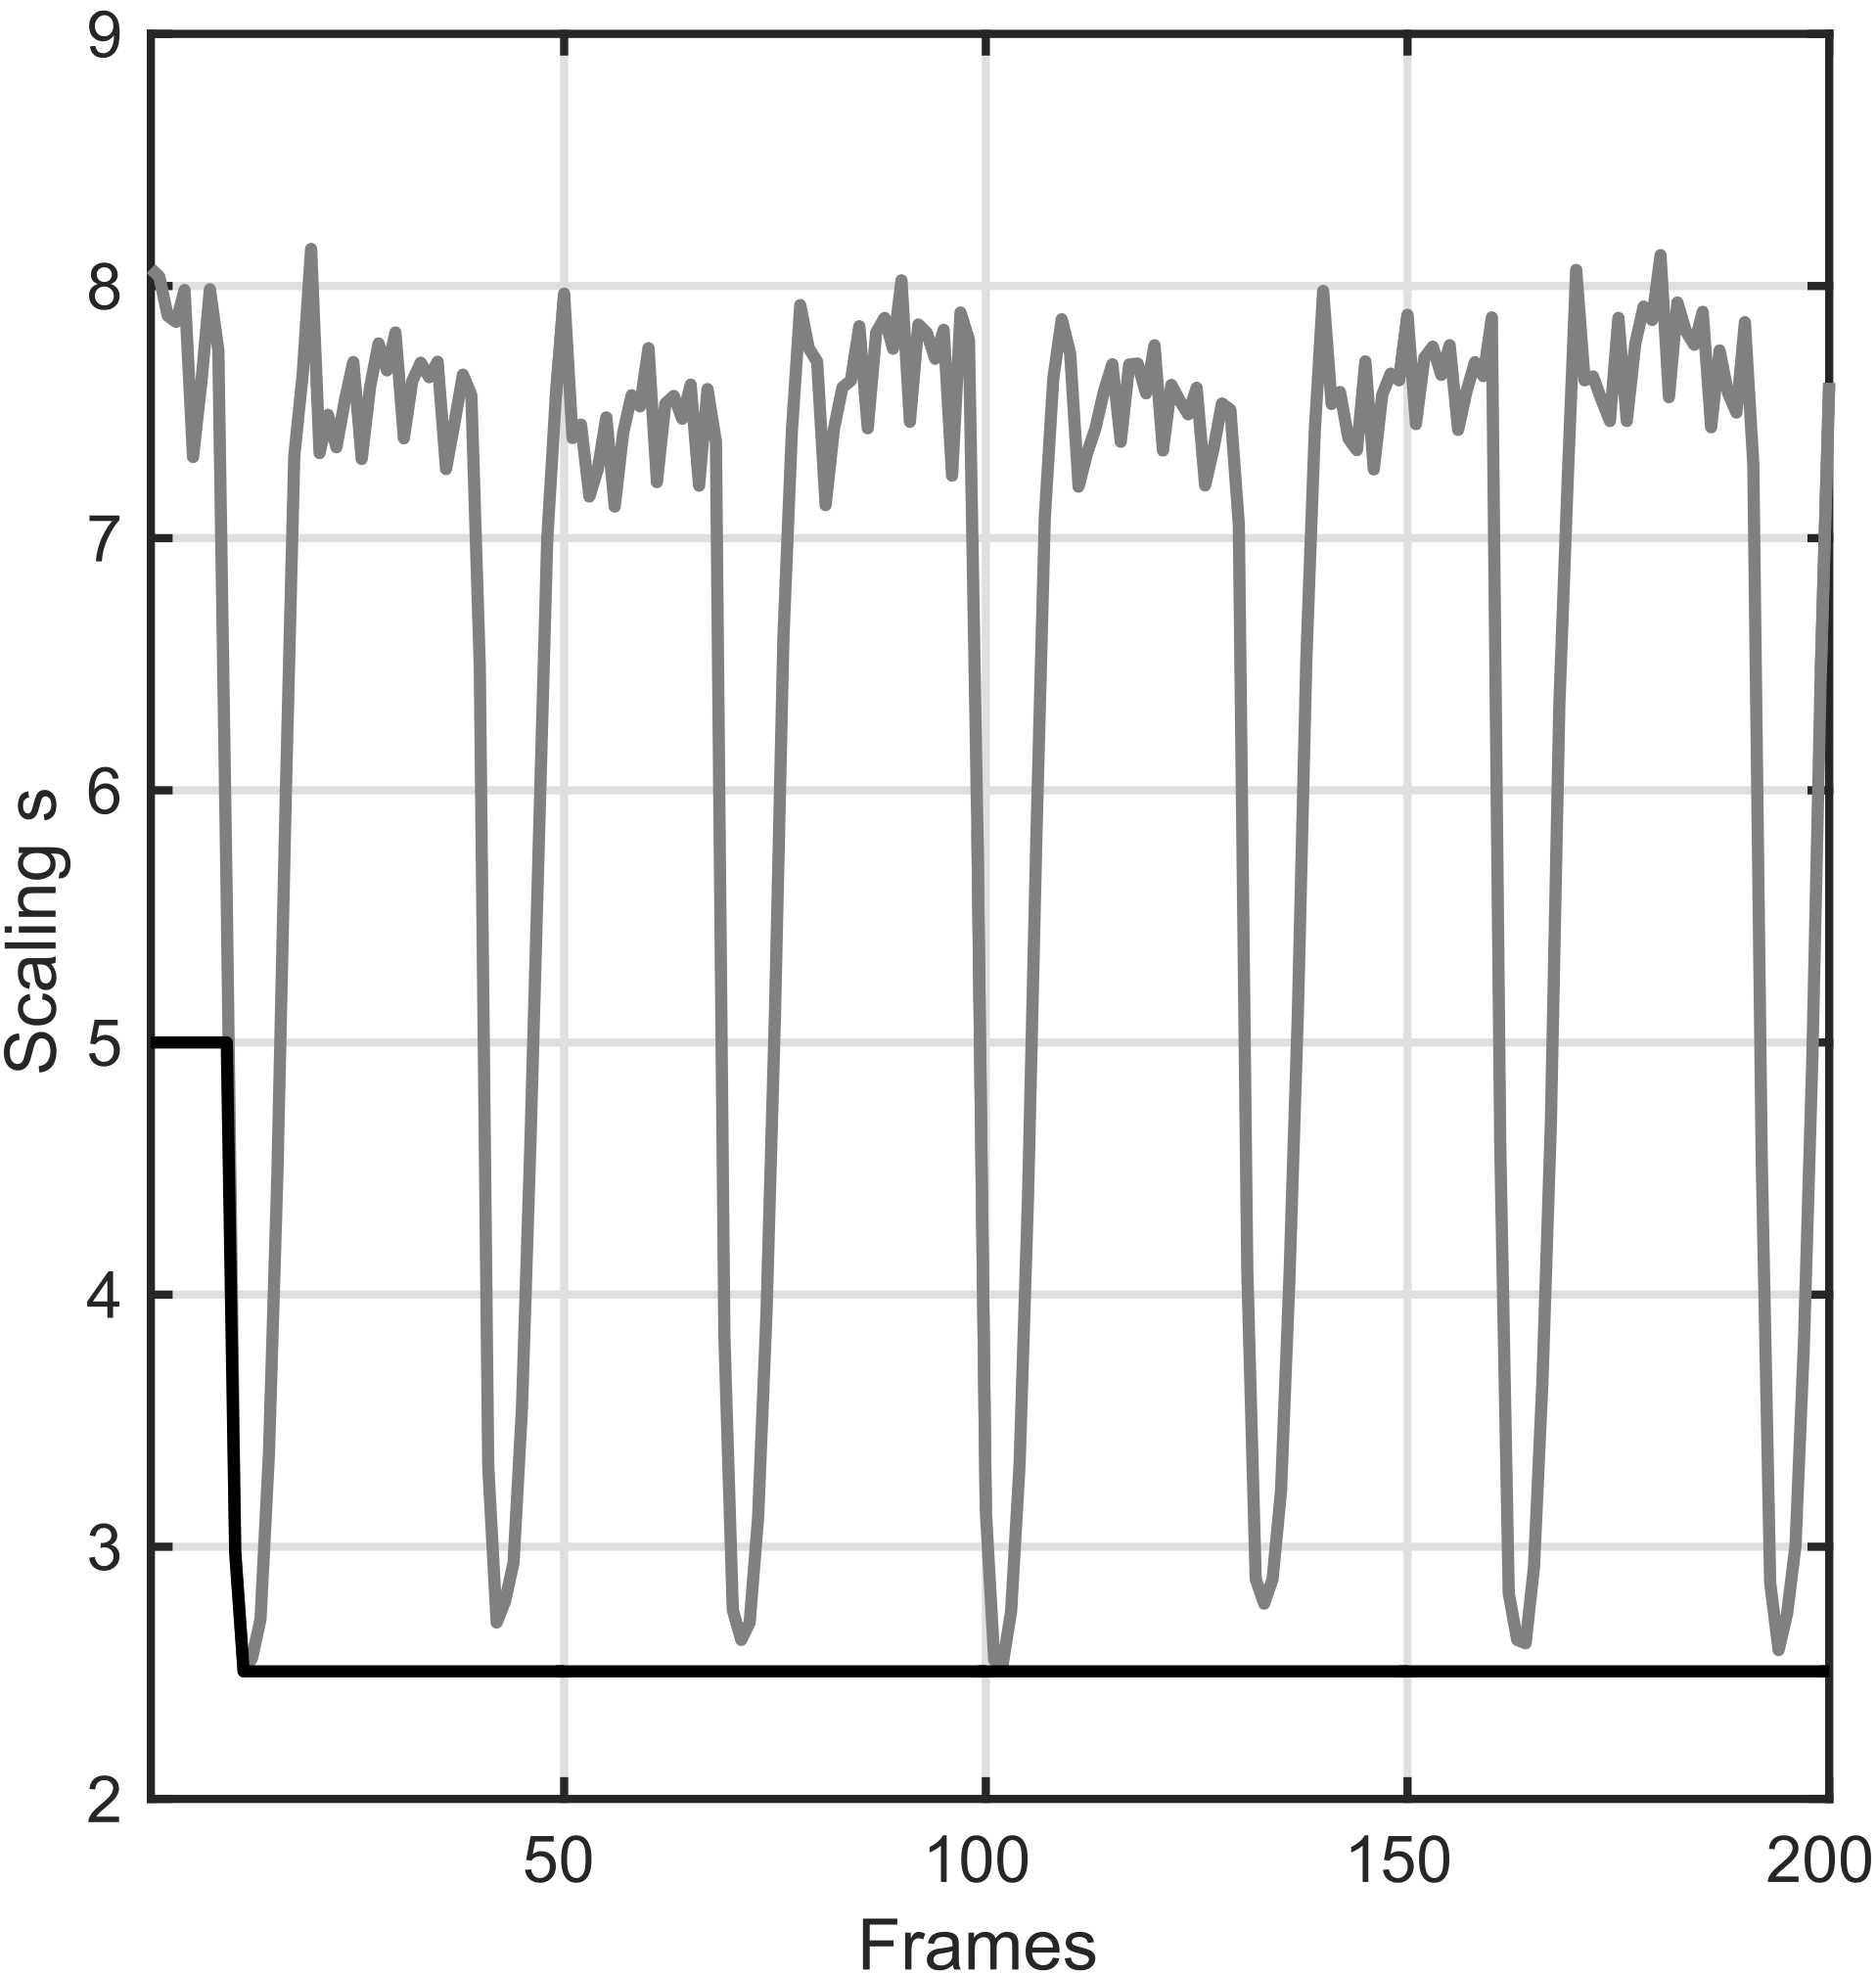
\includegraphics[width=0.8\textwidth]{fig/mir-pc-scaling.png}
  \caption{The scaling values $s$ for real-time phase-contrast flow MRI (\SI{35.7}{\ms} resolution) of the aorta of a healthy subject: Gray line $=$ according to \cref{Equ:mir_pc_scaling}), black line $=$ used for serial model-based reconstructions.} \label{Fig:mir-pc-scaling}
\end{figure}

Because real-time phase-contrast flow MRI is a dynamic process, serial phase-difference maps (as well as complex-difference images) may lead to different scaling values as determined by \cref{Equ:mir_pc_scaling}. This variation is shown in \cref{Fig:mir-pc-scaling} for experimental data of the human aorta (gray line). While $s$ can be as large as \num{10} in case of very low phase-difference values, i.e. in the absence of flow, such large values should be avoided as they decrease the regularization strength and accumulate noise in the final estimate. Therefore, the following steps are taken to dynamically determine the effective scaling. Starting with a value of \num{5}, $s$ is calculated from \cref{Equ:mir_pc_scaling} for each frame and continuously updated by any lower scaling. For studies of human blood flow this typically means that $s$ decreases until the real-time flow MRI acquisition reaches the first systole (compare \cref{Fig:mir-pc-scaling}, black line), so that quantitative analyses of real-time flow MRI studies may eliminate the first cardiac cycle.


\subsection{Regularization}
As shown in \cref{Equ:CG_cost}, Tikhonov regularization is used for the solution of the linear problem with $\alpha_n$ a tunable regularization parameter, which starts with \num{1} and decreases in each Newton step by a factor of \num{2}. In this study, $\alpha_n$ is identical among all parameters. In addition, the model-based image reconstruction adopts the $L^2$-norm regularization on the high spatial frequencies of the coil sensitivity maps as used for NLINV \cite{2010_20ms_Uecker,2008_NLINV,2010_NLINV_Heart,2012_PC_Joseph,2014_PC_Joseph,2015_PC_Asym}, and employs a temporal regularization of the current set of model parameters (i.e., maps) with the respective maps of the immediately preceding pair of datasets damped by \num{0.7}. The reconstruction on the very first maps is initialized using $\rho=1$, $z=0$, and $c_j=0$, and \num{7} Newton steps are used in this work.

The radial sampling pattern has a circular field-of-view, and thus encodes no information in the corners of k-space. As a result, high spatial-frequency signal, which usually appears as checkerboard artifacts in image domain, has the freedom to accumulate during model-based iterative reconstruction. Therefore, a k-space filter \cite{2001_gSENSE} is added to the gridded sampling pattern P to penalize signals in the undefined corners of k-space.


\subsection{Pre- and Post-Processing}
In general, the datasets from multiple receiver coils are first corrected for gradient delay errors \cite{2015_PC_Asym}, and then compressed to \num{10} virtual coils by a principle component analysis. This latter process must be identical for both the flow-compensated and flow-encoded datasets. Finally, the data and the sampling trajectories are interpolated onto Cartesian grids without density compensation. After solving the nonlinear inverse problem, the resulting complex phase-contrast map is given by
\begin{equation} \label{Equ:post_PC}
  \rho_{PC} = \abs{\rho} \cdot e^{i \cdot s \cdot \Im(\hat{z})} \quad .
\end{equation}


\section{Methods}
\subsection{Numerical Flow Phantom}
To ensure the quantitative accuracy of the proposed reconstruction method, a numerical flow phantom was built with superimposed ellipses, whose analytical Fourier transform is known and can be evaluated at given k-space trajectories. Moreover, \num{10} receiver coils were simulated based on the Biot-Savart law and sinusoidal fitting \cite{2012_analSim}. To mimic phase-contrast flow MRI, the simulation included one flow-compensated and one flow-encoded acquisition with the same magnitude signal strengths. The simulated ellipses had zero phase in the flow-compensated acquisition, while phase values of \SI{150}{\degree}, \SI{-100}{\degree}, and \SI{-15}{\degree} were added to the three ellipses in the flow-encoded acquisition to represent different velocities and directions. The simulations were performed for datasets with \num{45}, \num{15}, \num{7} and \num{5} radial spokes (symmetric echoes, base resolution \num{170} pixels) each covering a view angle of \SI{360}{\degree}. Serial datasets employed interleaved spokes in \num{5} successive acquisitions similar to experimental conditions. Complex white Gaussian noise with a standard deviation of \num{0.1} was added to the data, so that the signal-to-noise ratio decreased with the number of spokes. While model-based image reconstructions of numerical phantoms which are based on analytical Fourier transform usually suffer from aliasing artifacts, these may be suppressed by decreasing the Tikhonov regularization parameter or by adjusting the sampling pattern \cite{2011_T2_Sumpf}. Here, a damping factor of \num{1} for the $z$ map was only used for reconstructions of the numerical flow phantom.


\subsection{Real-Time Phase-Contrast Flow MRI}
This work presents real-time flow MRI data of the ascending (and descending) aorta obtained at \SI{3}{\tesla} (Magnetom Prisma, Siemens Healthcare, Erlangen, Germany). The analyses include \num{5} volunteers without known illness and two patients with combined aortic valve insufficiency and partial stenosis previously studied with “conventional” real-time flow MRI \cite{2015_PC_Asym} as well as new experimental data from 5 additional healthy subjects. All subjects gave written informed consent prior to MRI in compliance with the regulations established by the local ethics committee. 

Real-time phase-contrast flow MRI was based on extremely undersampled radial FLASH MRI (\num{5} or \num{7} spokes per image) with asymmetric gradient echoes \cite{2015_PC_Asym} using two sequential acquisitions of a dataset with velocity-compensated gradients in all gradient axes and with velocity-encoding of through-plane flow, respectively. While studies of the experimental flow phantom ($\text{VENC} = \SI[per-mode=reciprocal]{200}{\cm\per\second}$) employed the 64-channel head coil, blood flow in the human aorta ($\text{VENC} = 200\text{ to }\SI{400}{\cm\per\second}$) was studied during free breathing by combining an 18-element thorax coil with 32 elements of the spine coil. Acquisitions (TR/TE = \num{2.38}/\SI{1.59}{\ms}, flip angle \SI{10}{\degree}) of the previously described flow phantom \cite{2015_PC_Asym} were performed at \SI{1.4}{\mm} in-plane resolution (\SI{192}{\mm} field-of-view, \SI{6}{\mm} slice thickness) and \SI{33.32}{\ms} temporal resolution (\num{7} spokes for the flow-encoded and flow-compensated image, respectively). All in vivo measurements (TE = \SI{1.70}{\ms}, flip angle \SI{10}{\degree}) had \SI{1.5}{\mm} in-plane resolution, \SI{320}{\mm} field-of-view, \SI{6}{\mm} slice thickness, and \SI{35.7}{\ms} (\num{2 x 7} spokes, TR = \SI{2.55}{\ms}) or \SI{25.6}{\ms} temporal resolution (\num{2 x 5} spokes, TR = \SI{2.56}{\ms}) corresponding to \num{28} or \num{39} frames per second (fps), respectively. For both NLINV and model-based reconstructions the serial magnitude images were subject to a temporal median filter, whereas no temporal filter was applied to phase-contrast maps. 

Online reconstruction and display of real-time NLINV images was achieved by a parallelized version of the NLINV algorithm \cite{2012_Schaetz} and a bypass computer (sysGen/TYAN Octuple-\acs{GPU}, Sysgen, Bremen, Germany) equipped with two processors (CPU, SandyBridge E5-2650, Intel, Santa Clara, CA) and \num{8} graphics processing units (TITAN, NVIDIA, Santa Clara, CA). The system was fully integrated into the reconstruction pipeline of the commercial MRI system. Depending on image matrix (i.e., resolution and/or FOV) the current reconstruction speed ranges from \num{6} to \num{14} fps (i.e., magnitude images and phase-contrast maps). At this stage, the model-based reconstruction was implemented on a single graphics processing unit (GeForce GTX 580, NVIDIA, Santa Clara, CA) and performed offline after data acquisitions. Typically, the current implementation takes about \SI{4.5}{\second} per frame.

Quantitative analyses of phase-contrast flow MRI data were obtained with the use of CAIPI prototype software (Fraunhofer MEVIS, Bremen, Germany), especially modified for the automated analysis of real-time MRI data, i.e., vessel or myocardial segmentation throughout the entire time series without the need for manual corrections \cite{2014_img_segment}.

\clearpage


\section{Results}
\subsection{Validation Studies}
In order to assess the quantitative reliability of the model-based phase-contrast flow MRI technique, the mathematical approach was validated with the use of a numerical flow phantom providing ground truth in the presence of noise. \cref{Fig:mir-pc-sim-pha} compares the results obtained for NLINV reconstructions with subsequent calculation of a phase-difference map and direct model-based reconstructions for simulations with a decreasing number of spokes per image. For high degrees of undersampling, the model-based phase-contrast maps present with visibly better signal-to-noise ratio and sharper “vessel” definition. The quantitative analyses in \cref{Tab:mir-pc-sim-pha} confirm the excellent accuracy of phase (i.e., velocity) values obtained by the proposed model-based reconstruction – even for acquisitions with only \num{7} or \num{5} spokes per image. Most importantly, this not only applies to mean values, but also to the standard deviations which for highly undersampled acquisitions are much smaller than for NLINV-based reconstructions.

Similarly, \cref{Fig:mir-pc-exp-pha} shows the results for an experimental phantom providing constant flow at two different velocities (i.e., depending on tube diameter) and two opposing flow directions (forward vs backward flow). Again, the most apparent feature is the almost noise-less appearance of the model-based phase-contrast map which benefits from the a priori knowledge of zero phase for all pixels without flow or no MRI signal. In contrast, all “conventional” flow MRI techniques, which rely on the phase-difference calculation of two independent complex images with differential flow encodings, yield arbitrary phase values (and corresponding phase differences) in zero-signal pixels as well as some tissue-dependent phase in pixels with stationary signal. In relation to this advantageous zero-phase property, which is effective as an additional constraint, the model-based reconstruction reduces the strength of residual streakings extending from the high-flow tubes in the phase-contrast maps shown in \cref{Fig:mir-pc-exp-pha}.

Most importantly, however, model-based phase-contrast maps yield a spatially much more accurate definition of the flow signal (i.e., vessel lumen) than obtainable by conventional NLINV reconstructions. In fact, the spatial information of the model-based phase-contrast map in \cref{Fig:mir-pc-exp-pha} precisely matches the magnitude image information, whereas flow areas in NLINV phase-contrast maps are larger compared to both the true lumen sizes. These qualitative observations are confirmed by quantitative analyses summarized in \cref{Tab:mir-pc-exp-pha}. In contrast to NLINV, model-based reconstructions not only yield almost identical flow areas in magnitude images and phase-contrast maps, but are also in close agreement with estimates of tube sizes as obtained by high-resolution MRI. Nevertheless, flow evaluations reveal good agreement between both flow MRI methods with respect to peak velocity as a direct (though focal) result of the phase-contrast determination, while flow volumes tend to be slightly larger than a determination by a flow meter.
\vspace{10mm}

\begin{figure}[h!]
  \centering
  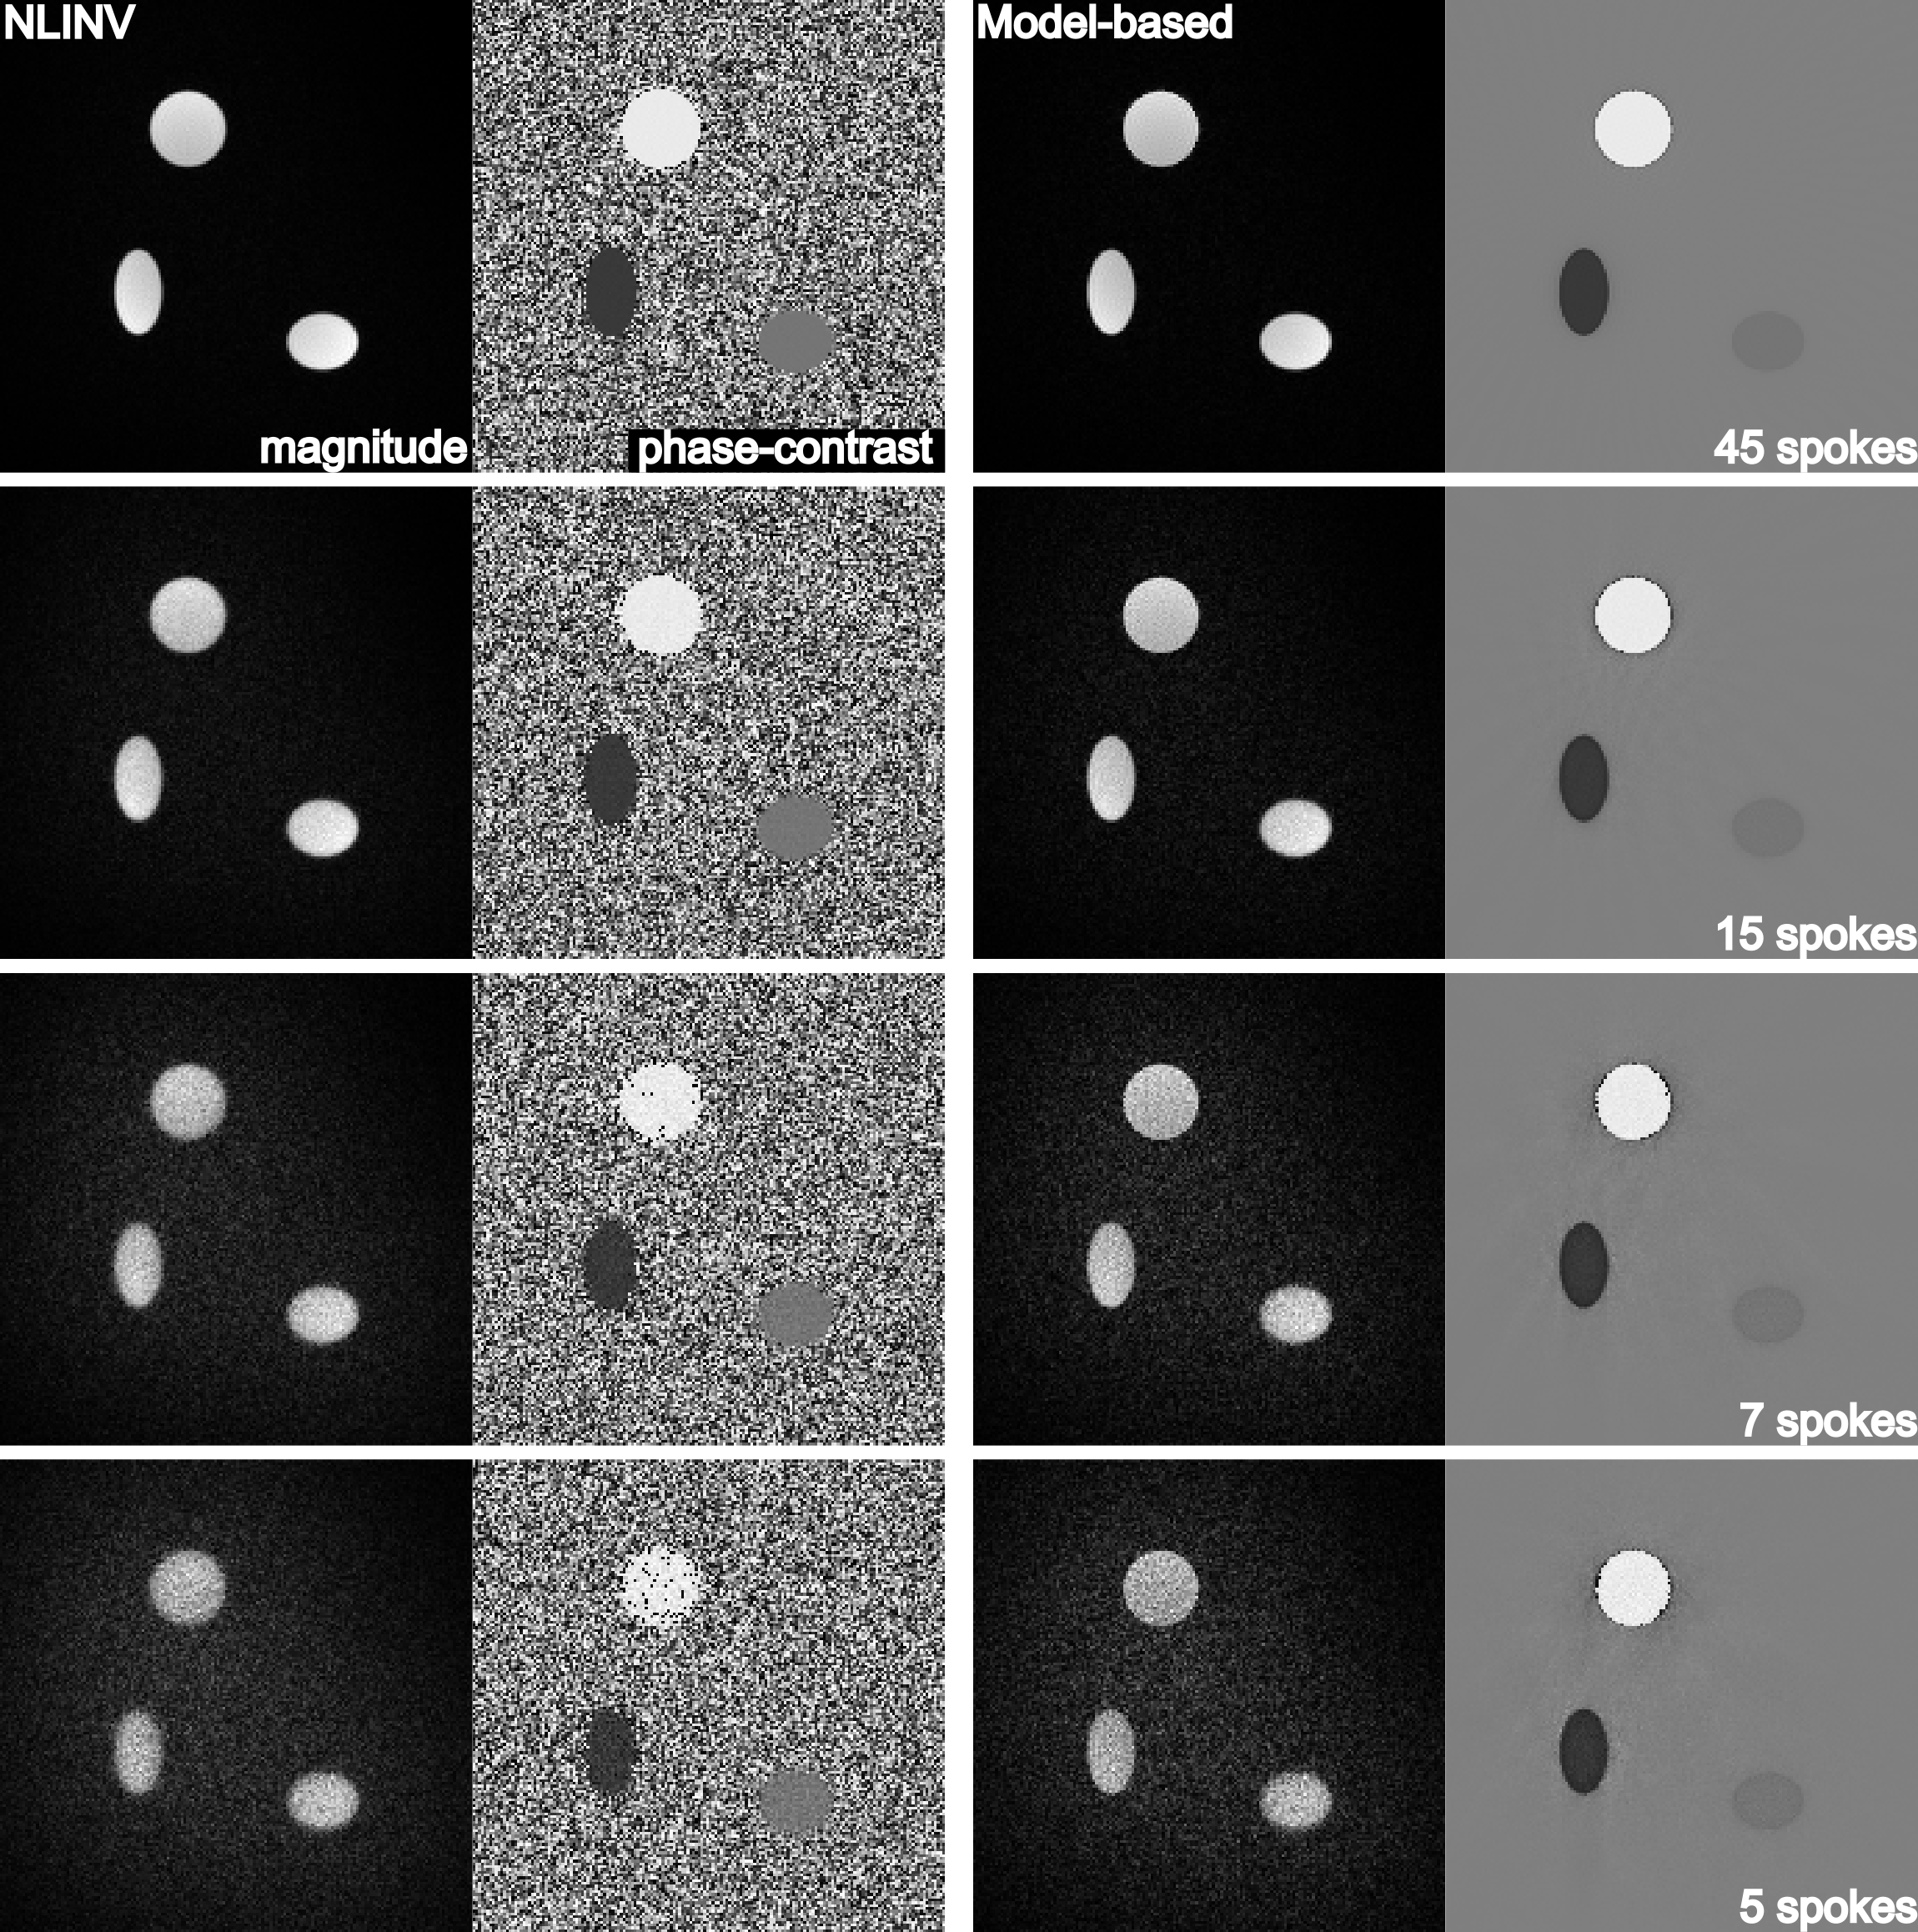
\includegraphics[width=\textwidth]{fig/mir-pc-sim-pha.png}
  \caption{(Left) NLINV and (right) model-based reconstructions of magnitude images and phase-contrast maps for a numerical flow phantom (complex white Gaussian noise, standard deviation \num{0.1}) and constant flow in three ellipses corresponding to phase values of \ang{150}, \ang{-100}, and \ang{-10}. The results were obtained for simulated acquisitions with \num{45}, \num{15}, \num{7} and \num{5} spokes. The Gibbs ringing artifact around the \ang{150} ellipse in phase-contrast maps stems from the numerical design of the phantom (plug flow pattern). It is less visible in NLINV reconstructions because of the phase noise for zero-flow pixels.} \label{Fig:mir-pc-sim-pha}
\end{figure}

\begin{table}[tb]
  \caption{Quantitative flow evaluations for a numerical flow phantom}
  \label{Tab:mir-pc-sim-pha}
  \begin{center}
    \begin{threeparttable}
      \begin{tabular}{ 	c 
					    S[table-format=-3]
					    S[table-format=-3.1(2)]
					    S[table-format=-3.1(2)] 
				     }
        \toprule
        {Spokes per image} & {True Phase Difference} & {NLINV\textsuperscript{1}} & {Model-based\textsuperscript{2}} \\
		\midrule
        \multirow{3}{*}{\tablenum[table-format=2]{45}} & 150  & 150.0\pm1.7   & 150.1\pm1.4  \\
                                                       & -100 & -100.0\pm1.4  & -100.2\pm1.0 \\
                                                       & -15  & -15.0\pm1.3   & -15.1\pm0.6  \\
        \hline
	    \multirow{3}{*}{\tablenum[table-format=2]{15}} & 150  & 150.0\pm5.5   & 149.8\pm2.5  \\
		                                               & -100 & -100.0\pm5.2  & -100.2\pm2.3 \\
		                                               & -15  & -15.0\pm4.4   & -15.0\pm1.6  \\
	    \hline
		\multirow{3}{*}{\tablenum[table-format=2]{7}}  & 150  & 146.4\pm36.0  & 149.6\pm5.7  \\
	                                                   & -100 & -100.8\pm12.0 & -102.7\pm5.3 \\
	                                                   & -15  & -15.6\pm10.6  & -15.5\pm3.1  \\
	    \hline
	    \multirow{3}{*}{\tablenum[table-format=2]{5}}  & 150  & 131.7\pm73.8  & 150.6\pm8.8  \\
		                                               & -100 & -101.6\pm18.6 & -103.8\pm6.5 \\
		                                               & -15  & -15.4\pm14.5  & -15.9\pm3.7  \\
	    \bottomrule
      \end{tabular}
  
      \begin{tablenotes}
	    \small
	    \item Results represent mean values $\pm$ standard deviations.
	    \item[1] NLINV reconstructions with subsequent calculation of a phase-different map.
	    \item[2] Direct model-based reconstruction of phase-contrast map.
	  \end{tablenotes}
    \end{threeparttable}
  \end{center}
\end{table}


\begin{figure}[tb]
  \centering
  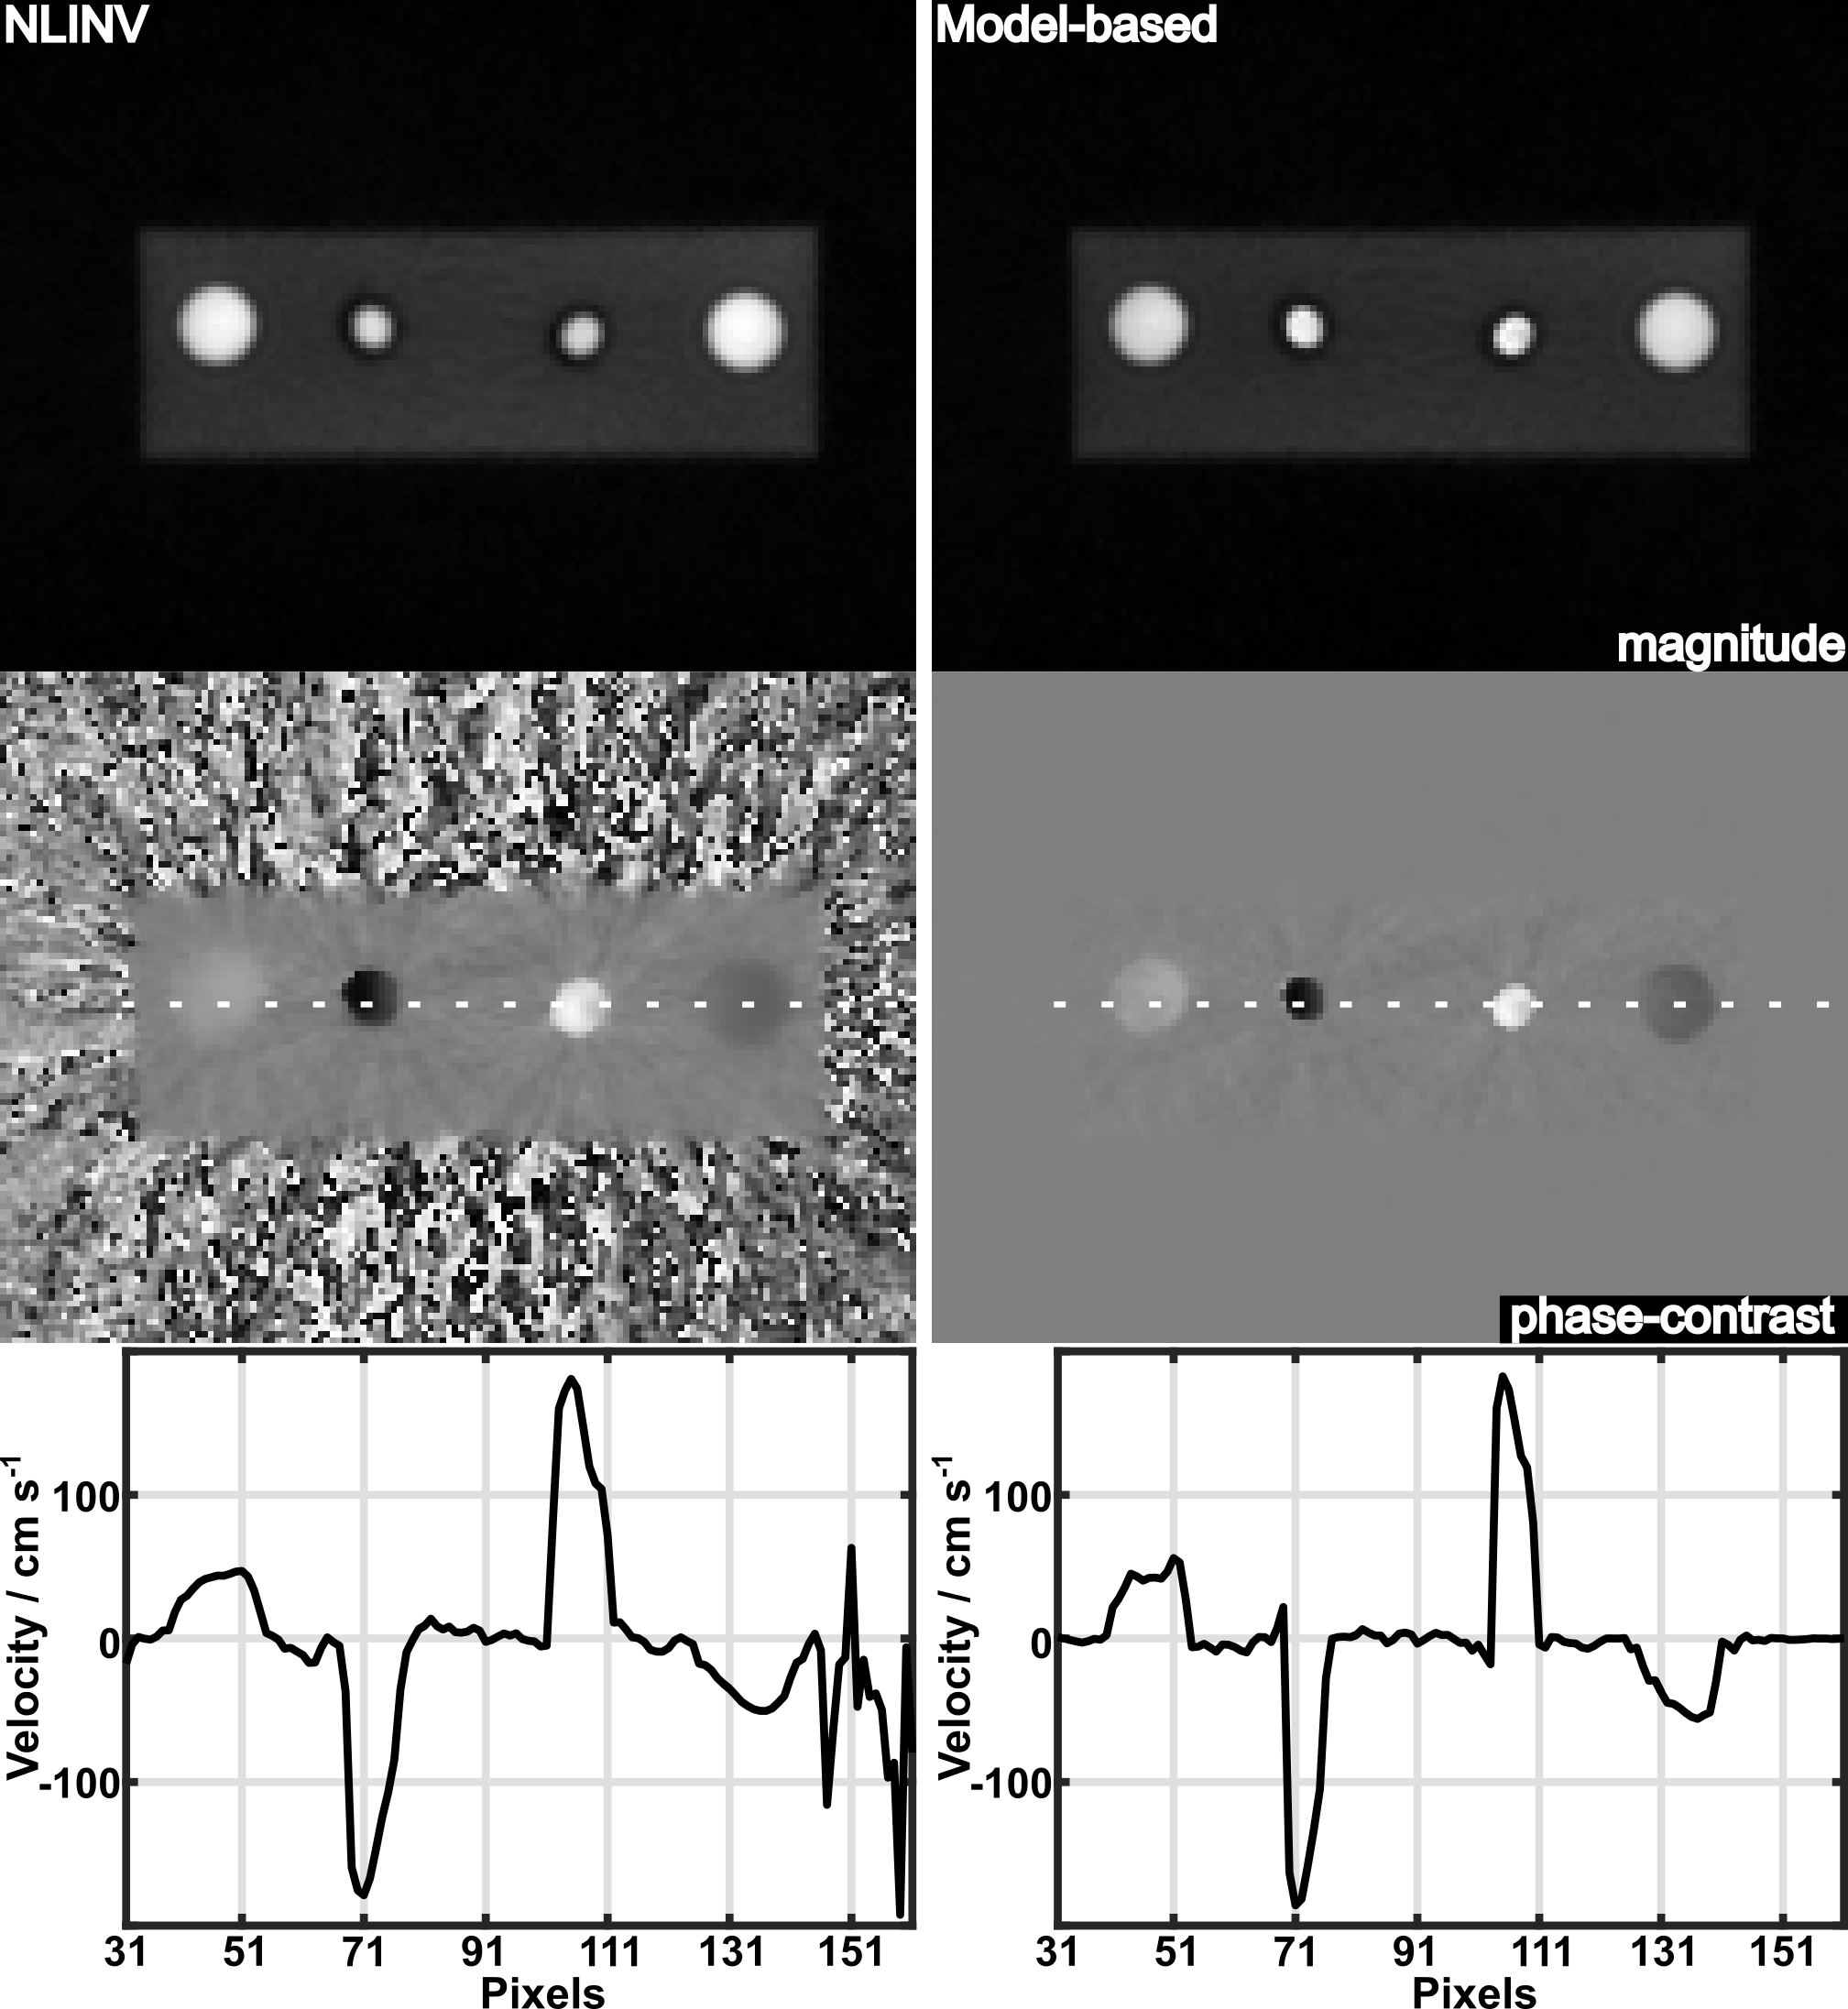
\includegraphics[width=0.8\textwidth]{fig/mir-pc-exp-pha.png}
  \caption{(Left) NLINV and (right) model-based reconstructions of (top) magnitude images and phase-contrast maps as well as (bottom) velocity profiles (along indicated reference lines) for an experimental flow phantom with constant (bidirectional) flow (tubes No.1 to No.4 from left to right, compare \cref{Tab:mir-pc-exp-pha}). The results were obtained for real-time phase-contrast flow MRI at \SI{33.3}{\ms} resolution and $\text{VENC} = \SI{200}{\cm\per\second}$. Residual streaking artifacts in the NLINV phase-contrast map are reduced in the model-based reconstruction which further improves the spatial definition of all tubes (compare \cref{Tab:mir-pc-exp-pha}).} \label{Fig:mir-pc-exp-pha}
\end{figure}

\begin{table}[tb]
  \caption{Quantitative evaluations of an experimental flow phantom}
  \label{Tab:mir-pc-exp-pha}
  \begin{center}
	\begin{threeparttable}
	  \begin{tabular}{ c 
					   c 
					   S[table-format=3] 
					   S[table-format=3] 
					   S[table-format=-3] 
					   S[table-format=-1.1] 
					 }
		\toprule
	    \multirow{3}{*}{{Tube\textsuperscript{1}}} & \multirow{3}{*}{{Method}} & {Magnitude} & {Phase-Contrast} & {Peak} & {Flow} \\
	     & & {Image\textsuperscript{2}} & {Map}               & {Velocity}              & {Volume\textsuperscript{3}} \\
         & & {(\si{\square\mm})}        & {(\si{\square\mm})} & {(\si{\cm\per\second})} & {(\si{\L\per\minute})} \\
	    \midrule
	    \multirow{2}{*}{No.1} & NLINV       & 255 & 360 & 55   & 6.5  \\
                              & Model-based & 239 & 243 & 63   & 6.8  \\
	    \hline
	    \multirow{2}{*}{No.2} & NLINV       & 76  & 131 & -189 & -7.3 \\
		                      & Model-based & 71  & 75  & -180 & -6.5 \\  
	    \hline
	    \multirow{2}{*}{No.3} & NLINV       & 78  & 139 & 181  & 6.9  \\
	                          & Model-based & 73  & 75  & 185  & 6.9  \\  
	    \hline
	    \multirow{2}{*}{No.4} & NLINV       & 255 & 302 & -52  & -7.0 \\
	                          & Model-based & 235 & 233 & -58  & -6.8 \\
	    \bottomrule
	  \end{tabular}
  
	  \begin{tablenotes}
	    \small
	    \item[1] Tube No.1 to No.4 are shown in \cref{Fig:mir-pc-exp-pha}.
	    \item[2] Estimated tube sizes from high-resolution MRI are about \SI{250}{\square\mm} (No.1, No.4) and \SI{70}{\square\mm} (No.2, No.3).
	    \item[3] The flow volume as determined by a flow meter was \SI{6.3}{\L\per\minute}.
	  \end{tablenotes}
    \end{threeparttable}
  \end{center}
\end{table}

\clearpage

\subsection{Human Studies}
Qualitative comparisons of NLINV and model-based phase-contrast MRI are depicted in \cref{Fig:mir-pc-vol-7s} for a normal subject and in \cref{Fig:mir-pc-pat} for a patient with aortic valve insufficiency and partial stenosis, respectively. In line with results for the experimental flow phantom, the systolic phase-contrast maps obtained by the model-based reconstruction yield a much better spatial definition in regions with non-zero flow (i.e., vessels). Here, this particularly applies to the descending aorta whose phase-difference presentation is in close agreement with the vessel lumen in the magnitude image. In quantitative terms the analysis of peak systolic frames from 10 consecutive heartbeats of the subject shown in \cref{Fig:mir-pc-vol-7s} revealed \SI{445+-16}{\square\mm} (\SI{781+-20}{\square\mm}) for the lumen of the descending (ascending) aorta in model-based phase-contrast maps vs \SI{569+-41}{\square\mm} (\SI{880+-18}{\square\mm}) for NLINV reconstructions.

In addition, the implicit a priori knowledge of zero phase in pixels without flowing spins precludes the iterative optimization process to generate residual streaking artifacts in areas around vessels with maximum systolic flow, i.e. for signals with high temporal and spatial frequencies that are most severely affected by k-space undersampling. Quantitative results for both NLINV and model-based reconstructions are summarized in \cref{Tab:mir-pc-old-dat} for 5 subjects and 2 patients studied previously \cite{2015_PC_Asym} and found to be in general agreement. In comparison to \cite{2015_PC_Asym} all analyses were performed with an extended gradient-delay correction (unpublished results) and evaluated with an updated software package for automatic vessel segmentation (CAIPI Prototype Software). In more detail, while peak velocities obtained by NLINV and model-based reconstruction reveal excellent agreement, stroke volumes (and cardiac output) which rely on integrated velocities over space and time are slightly lower for model-based reconstructions. This observation reflects the sharper (i.e., smaller) definition of the vessel lumen and must not be considered a flaw but an advantage.

The spatiotemporal improvement achievable by model-based phase-contrast flow MRI may be invested into even faster acquisitions. As already suggested by the numerical simulations presented in \cref{Fig:mir-pc-sim-pha} and \cref{Tab:mir-pc-sim-pha}, \cref{Fig:mir-pc-vol-7s-5s} advances NLINV and model-based phase-contrast flow acquisitions from \num{7} spokes per image and \SI{35.7}{\ms} total acquisition time to \num{5} spokes and \SI{25.6}{\ms} resolution. At peak systole the findings of excellent vessel definition with almost no phase noise and residual streakings confirm the expectations from numerical and experimental validations. Together, these findings clearly support the notion that the use of \num{5} spokes represents an extreme but feasible approach to real-time flow MRI at high temporal resolution. This is further confirmed by the quantitative evaluations in \cref{Tab:mir-pc-new-dat} summarizing peak velocities and flow rates for \num{5} additional subjects and acquisitions with \num{7} and \num{5} spokes. Regardless of possible intrasubject variability in repetitive measurements, mean peak velocities and flow volumes (10 heartbeats) in both the ascending and descending aorta differ by less than \SI{4}{\percent} when comparing \SI{35.7}{\ms} acquisitions (\num{7} spokes) with \SI{25.6}{\ms} acquisitions (\num{5} spokes).
\vspace{10mm}

\begin{figure}[h!]
  \centering
  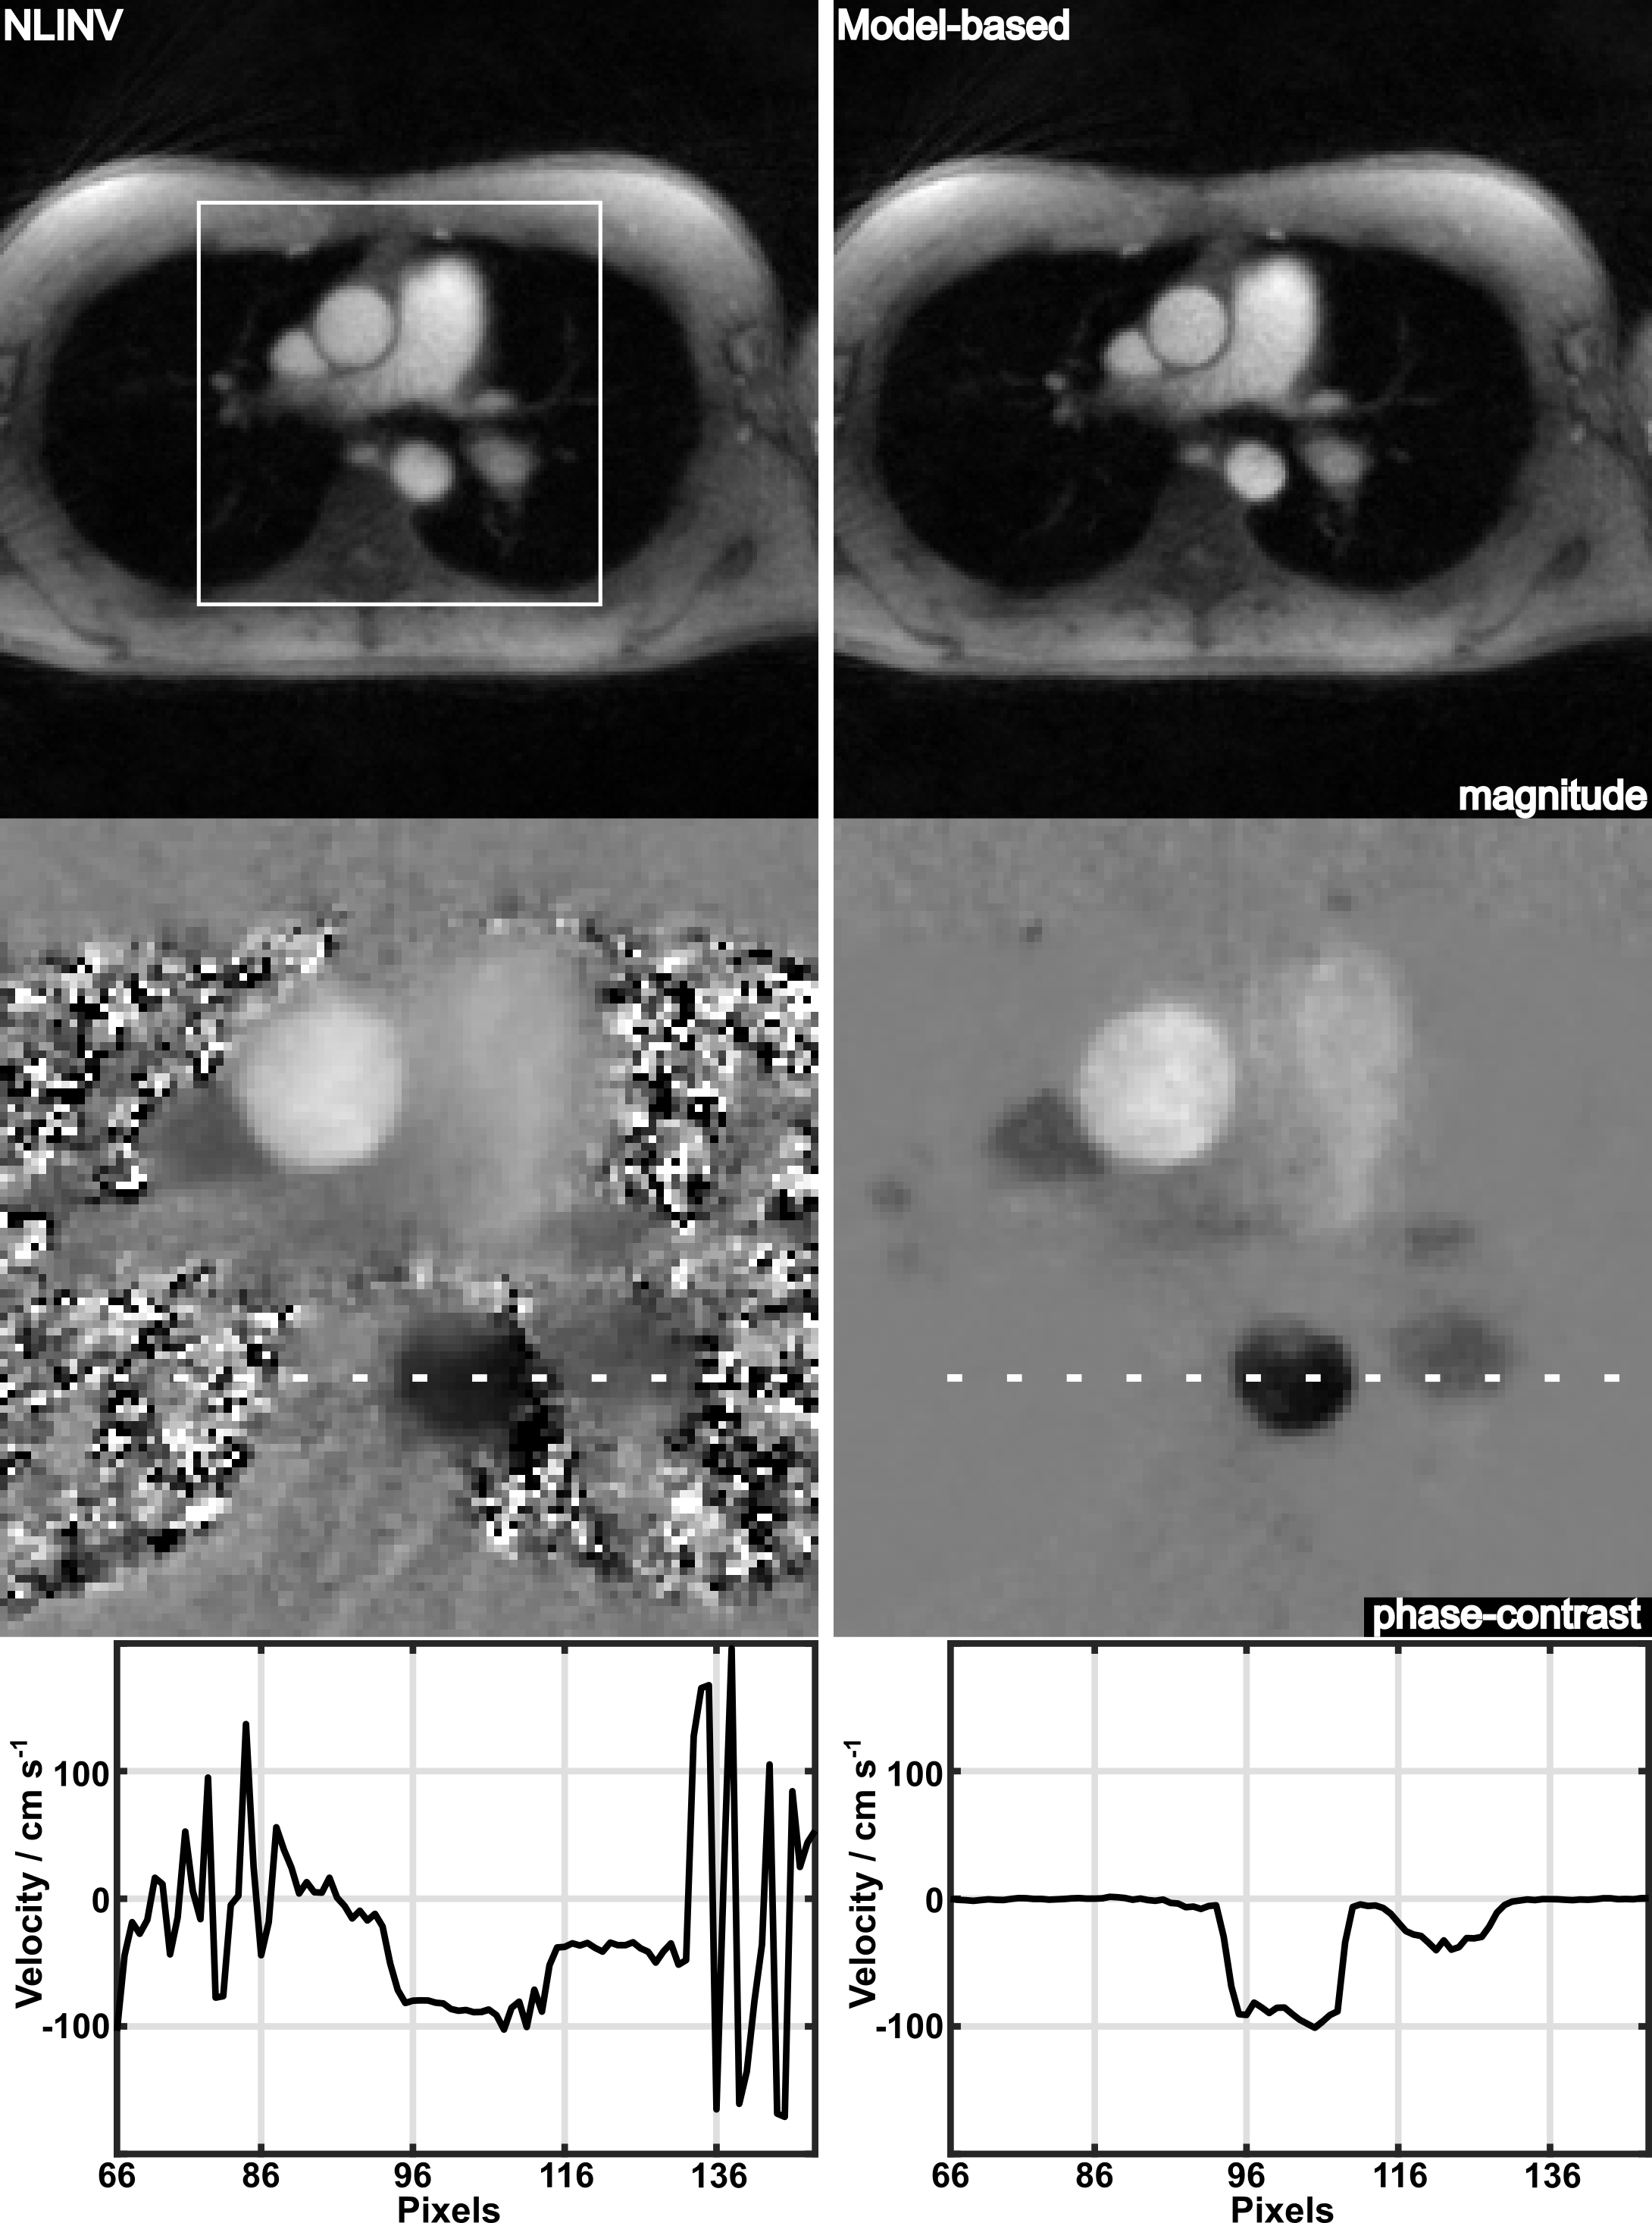
\includegraphics[width=0.8\textwidth]{fig/mir-pc-vol-7s.png}
  \caption{(Left) NLINV and (right) model-based reconstructions of (top) systolic magnitude images and phase-contrast maps (magnified views) as well as (bottom) velocity profiles (along indicated reference lines) for real-time phase-contrast MRI of aortic blood flow in a healthy volunteer at \SI{35.7}{\ms} resolution and $\text{VENC} = \SI{200}{\cm\per\second}$.} \label{Fig:mir-pc-vol-7s}
\end{figure}

\begin{figure}[tb]
  \centering
  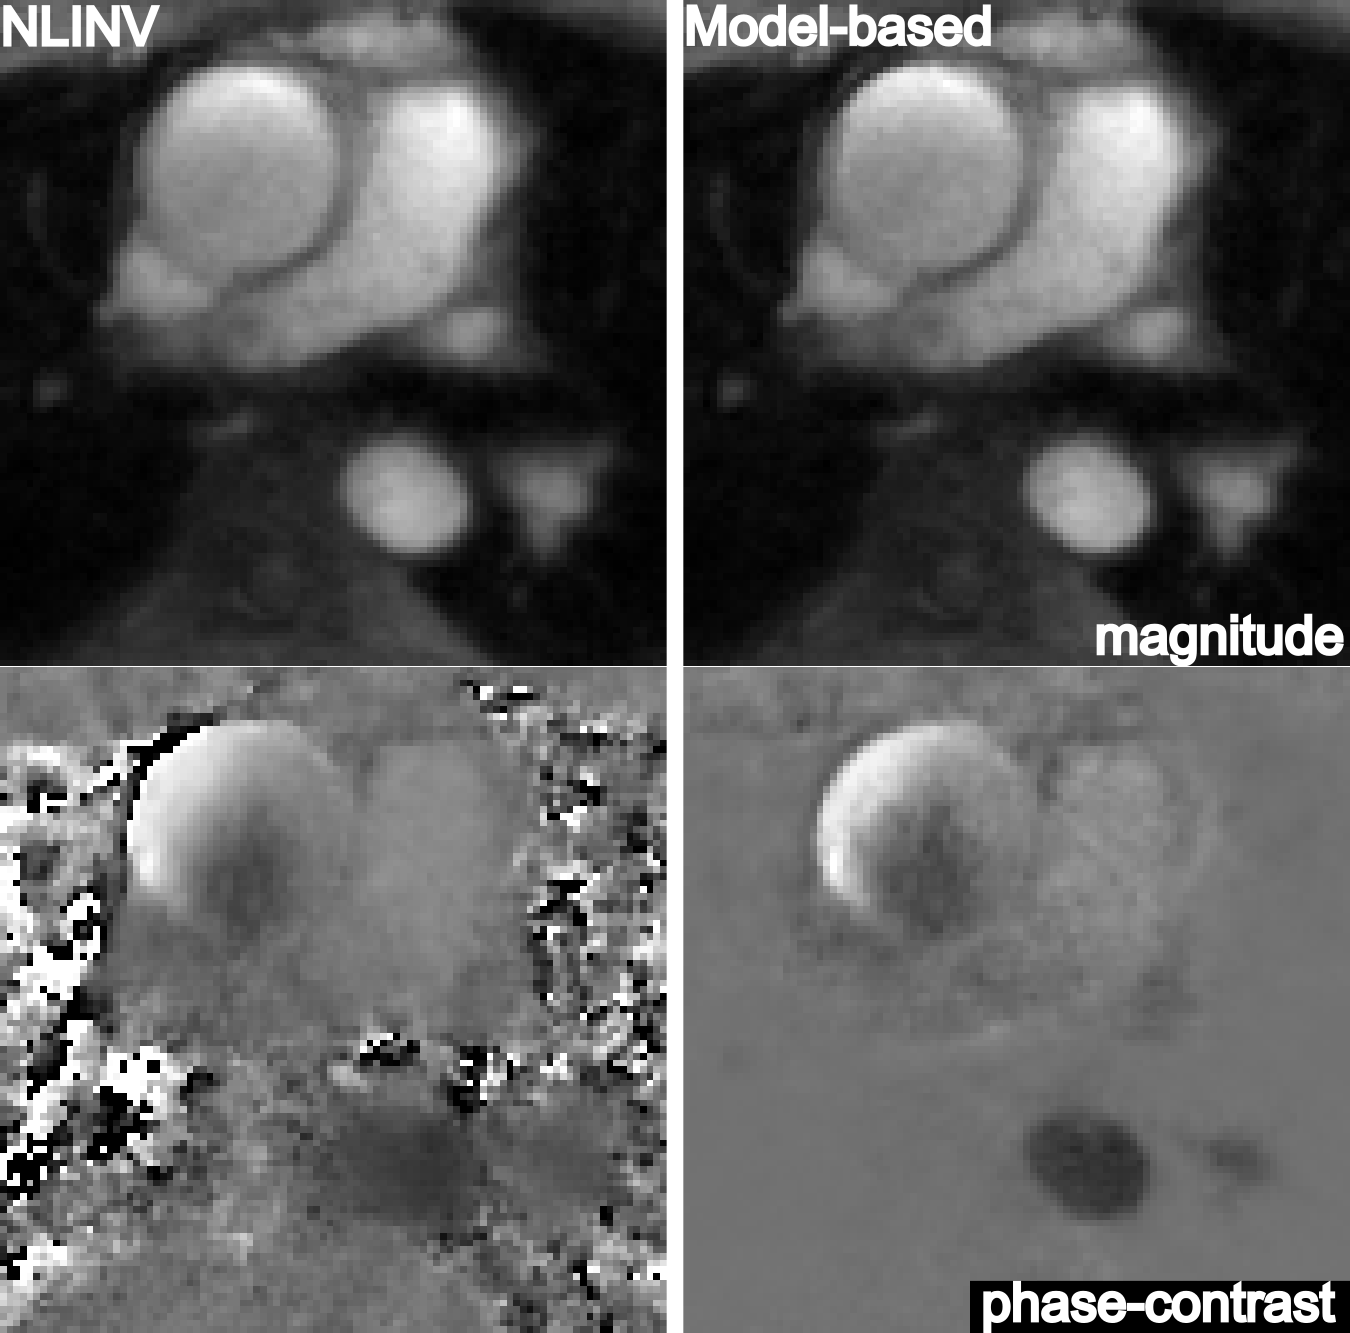
\includegraphics[width=0.80\textwidth]{fig/mir-pc-pat.png}
  \caption{(Left) NLINV and (right) model-based reconstructions of systolic magnitude images and phase-contrast maps (magnified views) for real-time phase-contrast MRI of a patient with aortic valve insufficiency and partial stenosis at \SI{35.7}{\ms} resolution and $\text{VENC} = \SI{400}{\cm\per\second}$.} \label{Fig:mir-pc-pat}
\end{figure}

\begin{table}[tb]
  \caption{Quantitative flow evaluations of the ascending aorta of healthy volunteers and patients with valve insufficiency (data from Ref.~\cite{2015_PC_Asym}). The results represent mean values $\pm$ standard deviation for \num{10} consecutive heartbeats at \SI{35.7}{\ms} resolution.}
  \label{Tab:mir-pc-old-dat}
  \begin{center}
	\begin{tabular}{ c 
					 c 
					 S[table-format=3(2)]
					 S[table-format=3(1)] 
					 S[table-format=1.1(2)] 
					 S[table-format=2(1)] 
				   }
	  \toprule
	  \multirow{3}{*}{Subject}   & \multirow{3}{*}{Method} & {Peak}                  & {Flow per}        & {Flow}                 & {Regurgitation}   \\
	                             &                         & {Velocity}              & {Heartbeat}       & {Volume}               & {Fraction}        \\
	                             &                         & {(\si{\cm\per\second})} & {(\si{\milli\L})} & {(\si{\L\per\minute})} & {(\si{\percent})} \\
	  \midrule
	  \multirow{2}{*}{No.1} & {NLINV}       & 120 \pm 3   & 99 \pm 4  & 5.7 \pm 0.4 & 2 \pm 1 \\
	                        & {Model-based} & 121 \pm 4   & 91 \pm 5  & 5.2 \pm 0.4 & 1 \pm 1 \\
	  \hline
	  \multirow{2}{*}{No.2} & {NLINV}       & 114 \pm 8   & 124 \pm 6 & 6.9 \pm 0.3 & 1 \pm 1 \\
	                        & {Model-based} & 114 \pm 7   & 112 \pm 5 & 6.3 \pm 0.2 & 1 \pm 1 \\
	  \hline
	  \multirow{2}{*}{No.3} & {NLINV}       & 69 \pm 3    & 61 \pm 3  & 4.0 \pm 0.2 & 2 \pm 1 \\
	                        & {Model-based} & 76 \pm 4    & 62 \pm 2  & 4.1 \pm 0.2 & 1 \pm 1 \\
	  \hline
	  \multirow{2}{*}{No.4} & {NLINV}       & 112 \pm 5   & 131 \pm 4 & 8.1 \pm 0.3 & 2 \pm 1 \\
	                        & {Model-based} & 111 \pm 4   & 123 \pm 4 & 7.6 \pm 0.3 & 2 \pm 1 \\  
	  \hline
	  \multirow{2}{*}{No.5} & {NLINV}       & 100 \pm 5   & 107 \pm 3 & 6.2 \pm 0.1 & 3 \pm 1 \\
	                        & {Model-based} & 109 \pm 5   & 97 \pm 3  & 5.6 \pm 0.1 & 4 \pm 1 \\
	  \hline
	  \multirow{2}{*}{Pat.1} & {NLINV}       & 264 \pm 14 & 56 \pm 6  & 3.0 \pm 0.3 & 55 \pm 3 \\
	                         & {Model-based} & 216 \pm 11 & 51 \pm 4  & 2.8 \pm 0.2 & 57 \pm 2 \\
	  \hline
	  \multirow{2}{*}{Pat.2} & {NLINV}       & 222 \pm 12 & 82 \pm 5  & 5.3 \pm 0.3 & 18 \pm 2 \\
	                         & {Model-based} & 219 \pm 6  & 71 \pm 6  & 4.6 \pm 0.4 & 23 \pm 3 \\
	  \bottomrule
	\end{tabular}
  \end{center}
\end{table}


\begin{figure}[tb]
  \centering
  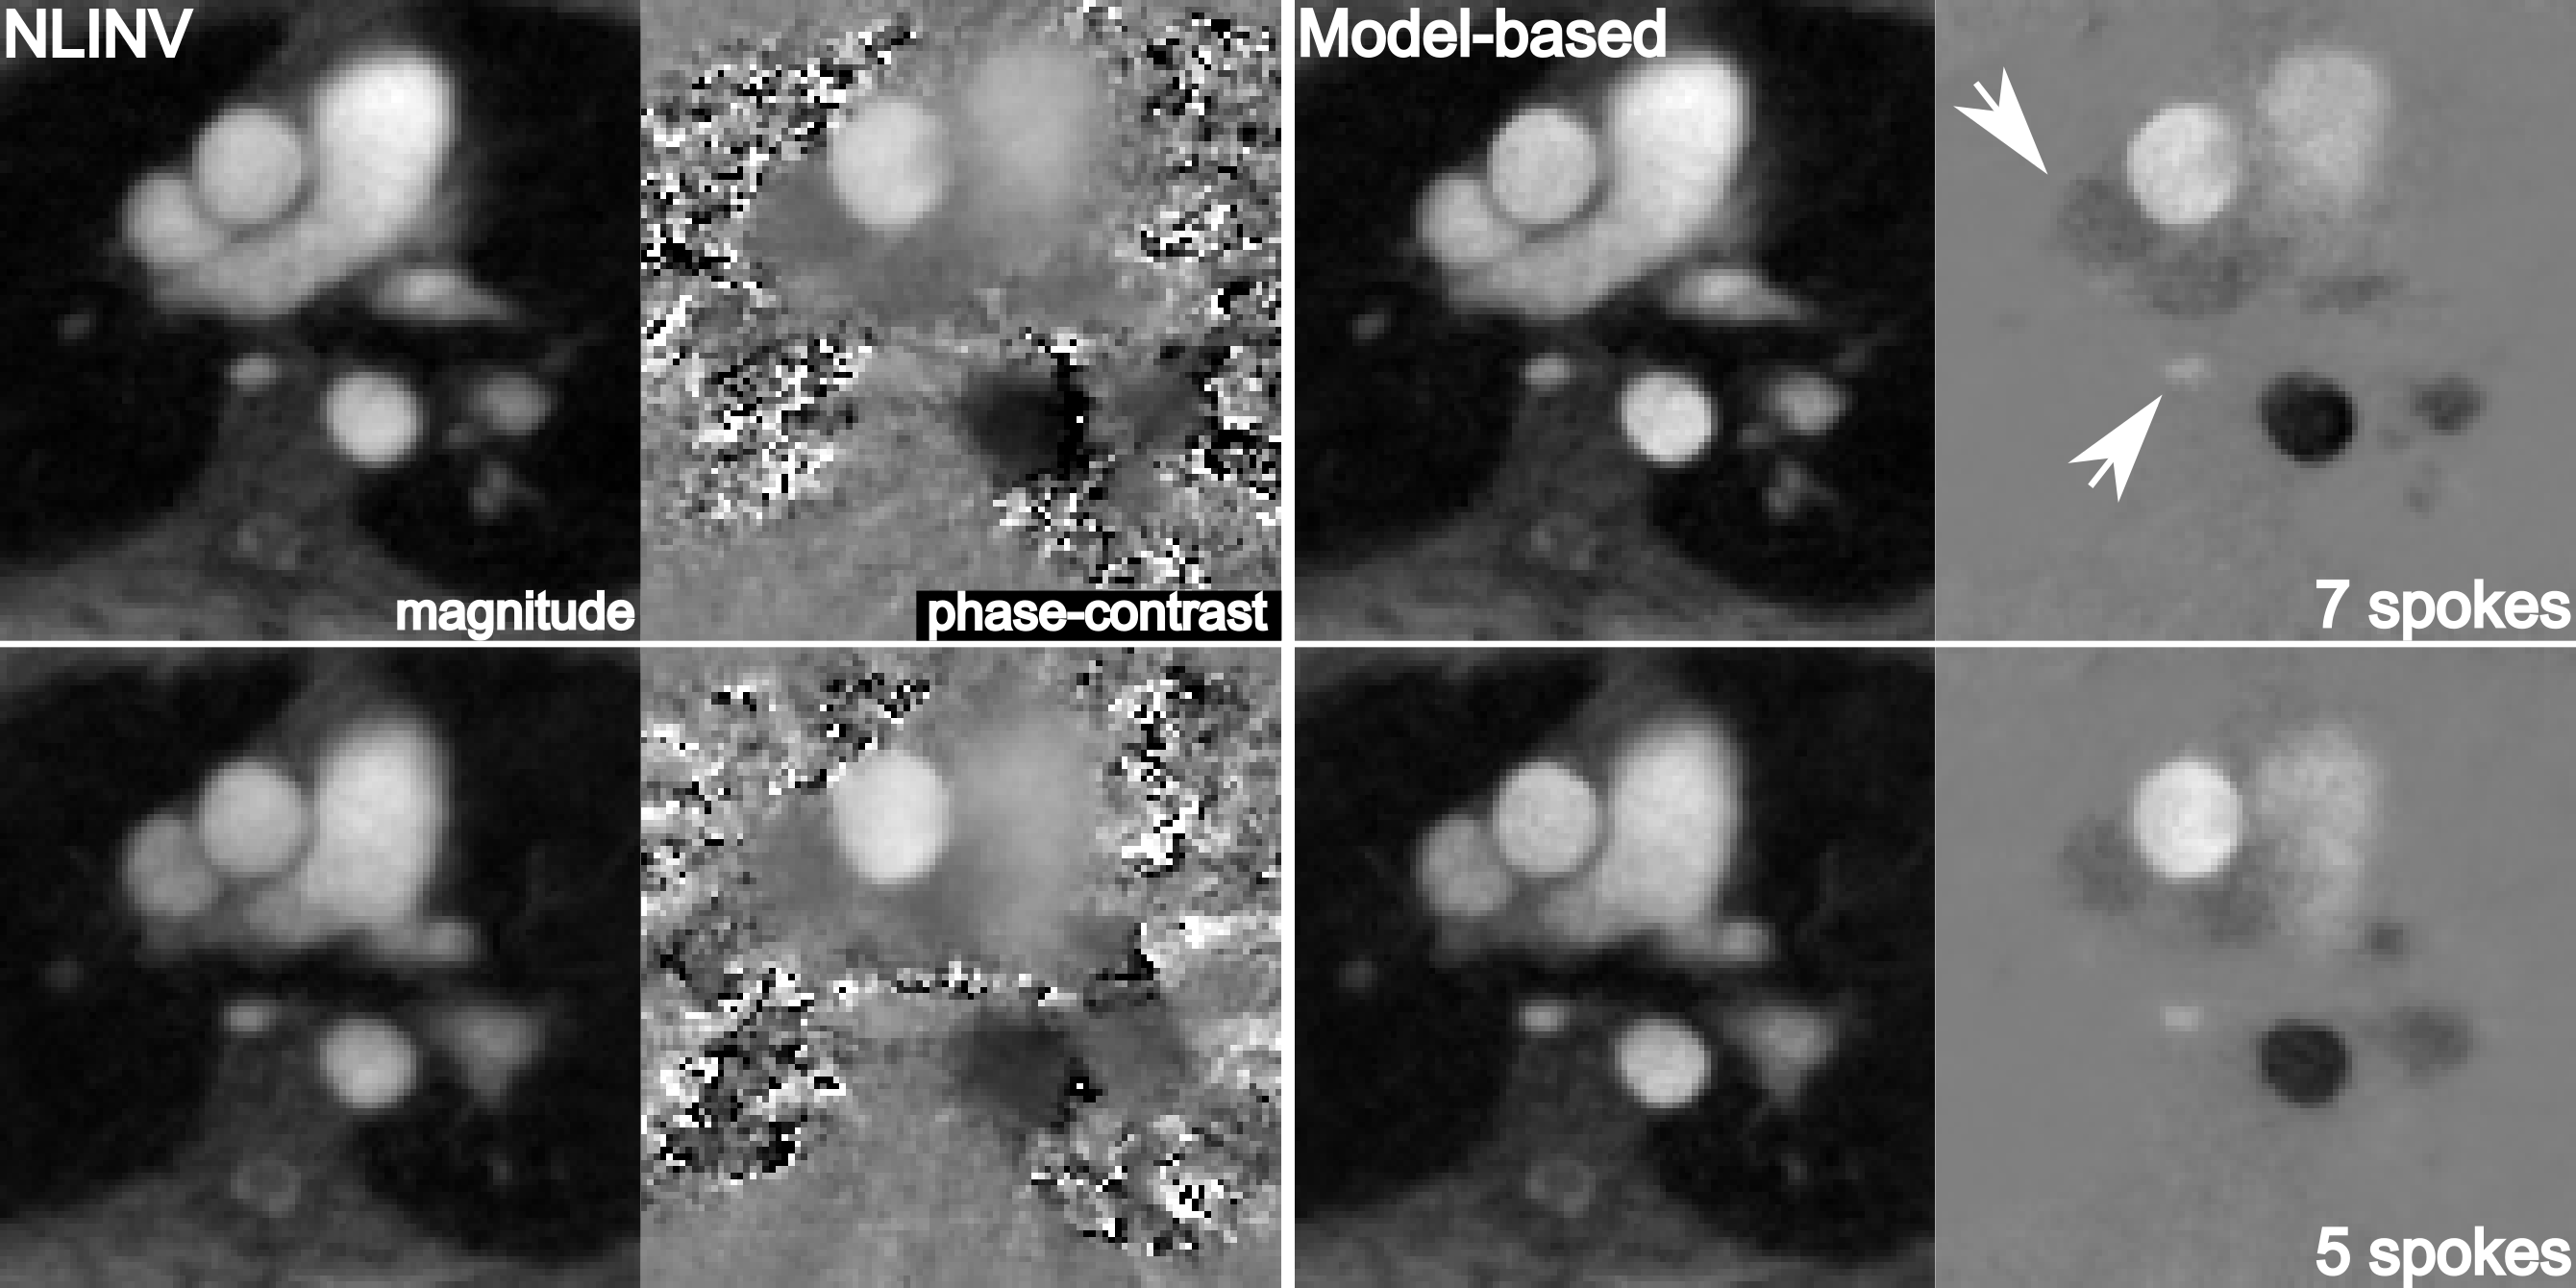
\includegraphics[width=\textwidth]{fig/mir-pc-vol-7s-5s.png}
  \caption{(Left) NLINV and (right) model-based reconstructions of systolic magnitude images and phase-contrast maps (magnified views) for real-time phase-contrast MRI of aortic blood flow (VENC = 200 cm s\textsuperscript{-1}) in a healthy volunteer using (top) 7 spokes per frame at 35.7 ms resolution and (bottom) 5 spokes at 25.6 ms resolution. Note the improved delineation of the superior vena cava (upper arrow) and the small azygos vein (lower arrow) in model-based phase-contrast maps.} \label{Fig:mir-pc-vol-7s-5s}
\end{figure}

\begin{table}[tb]
  \caption{Quantitative flow evaluations of model-based reconstructions in the ascending and descending aorta of healthy volunteers. The results represent mean values $\pm$ standard deviation for 10 consecutive heartbeats at \SI{35.7}{\ms} and \SI{25.6}{\ms} resolution, respectively. The bottom row presents percent differences of mean values for acquisitions at \SI{35.7}{\ms} and \SI{25.6}{\ms} resolution.}
  \label{Tab:mir-pc-new-dat}
  \begin{center}
	\begin{tabular}{ c 
					 c 
					 S[table-format=-3(2)] 
					 S[table-format=-3(1)] 
					 S[table-format=-3(1)] 
					 S[table-format=2(2)] }
	                           &          & \multicolumn{2}{c}{\textbf{Ascending Aorta}} & \multicolumn{2}{c}{\textbf{Descending Aorta}} \\
	  \toprule
	  \multirow{3}{*}{Subject} & {Spokes} & {Peak}                  & {Flow per}         & {Peak}                  & {Flow per}          \\
	                           & {per}    & {Velocity}              & {Heartbeat}        & {Velocity}              & {Heartbeat}         \\
	                           & {Image}  & {(\si{\cm\per\second})} & {(\si{\milli\L})}  & {(\si{\cm\per\second})} & {(\si{\milli\L})}   \\
	  \midrule
	  \multirow{2}{*}{No.6}    & 7        & 88 \pm 4  & 96 \pm 9  & 99 \pm 5  & 58 \pm 5 \\
	                           & 5        & 89 \pm 4  & 100 \pm 4 & 103 \pm 5 & 70 \pm 3 \\
	  \hline
	  \multirow{2}{*}{No.7}    & 7        & 127 \pm 6 & 107 \pm 6 & 128 \pm 5 & 81 \pm 4 \\
	                           & 5        & 116 \pm 6 & 94 \pm 5  & 120 \pm 6 & 68 \pm 4 \\
	  \hline
	  \multirow{2}{*}{No.8}    & 7        & 83 \pm 7  & 77 \pm 7  & 104 \pm 4 & 52 \pm 4 \\
	                           & 5        & 84 \pm 10 & 76 \pm 7  & 104 \pm 6 & 55 \pm 4 \\
	  \hline
	  \multirow{2}{*}{No.9}    & 7        & 114 \pm 3 & 106 \pm 4 & 119 \pm 3 & 60 \pm 3 \\
	                           & 5        & 115 \pm 2 & 103 \pm 5 & 115 \pm 3 & 60 \pm 4 \\
	  \hline
	  \multirow{2}{*}{No.10}   & 7        & 96 \pm 4  & 81 \pm 3  & 100 \pm 5 & 54 \pm 3 \\
	                           & 5        & 96 \pm 3  & 75 \pm 4  & 100 \pm 3 & 54 \pm 3 \\
	  \hline
	  {Diff. (\si{\percent})}  & 7 vs 5   & -1 \pm 4  & -4 \pm 6  & -1 \pm 4  & 2 \pm 13 \\
	  \bottomrule
    \end{tabular}
  \end{center}
\end{table}

\clearpage

\section{Discussion}
This work demonstrates the successful development of a model-based reconstruction technique for real-time phase-contrast flow MRI and its application to the assessment of cardiovascular blood flow. When compared to a previous flow MRI method based on NLINV reconstructions of two independent flow-compensated and flow-encoded images \cite{2015_PC_Asym}, the flow results are quantitatively accurate, while the images and maps present with improved spatial acuity and reduced residual streaking artifacts. Most importantly, the desired phase-difference maps reveal much reduced phase noise when compared to phase-difference maps of two complex images with arbitrary phases, in particular in areas of low or no MRI signal. As a consequence, the proposed method offers much better access to small vessels such as for example the azygos vein (see \cref{Fig:mir-pc-vol-7s-5s}). On the other hand, the improved image quality and vessel definition of the model-based phase-contrast method allows for the use of only \num{5} spokes per image which pushes flow MRI to a temporal resolution of \SI{25.6}{\ms} or a rate of \num{39} phase-contrast maps per second. Similar degrees of radial undersampling (i.e., \num{5} spokes per image) have already successfully been applied for real-time MRI studies of high-speed tongue movements in elite horn players \cite{2015_horn_QIM} and experimentally been demonstrated to provide excellent temporal fidelity for a rapid motion phantom \cite{2014_Temp_Fidelity} when eliminating any temporal filter as done here for the velocity-encoded phase-contrast maps.

At this time, the most relevant limitation of the proposed method is the need for a time-consuming offline calculation. Although conventional NLINV reconstructions are available online for immediate control \cite{2015_PC_Asym}, the nonlinear inverse problem posed by the phase-contrast flow MRI signal model requires new efforts for parallelization, GPU programming and implementation on the existing bypass server to the host computer of our MRI system. Nevertheless, such work will be mandatory to provide an online version for extended clinical trials. Another future option might be a comparative investigation of other model-based flow MRI methods and their applicability to highly undersampled MRI data. However, such studies are outside the scope of the present work, which offers multiple validations of the proposed model-based reconstruction for real-time flow MRI comprising numerical simulations, an experimental phantom, normal subjects and patients with previous ECG-synchronized flow MRI data \cite{2015_PC_Asym}.

An advantageous extension of the current model-based reconstruction may arise from the fact that the method is applicable to arbitrary trajectories in k-space, and in particular, to different spatial encodings (i.e., sets of spokes) for the flow-encoded and flow-compensated dataset. So far, most if not all phase-contrast MRI acquisition techniques including the one used here, employ the same lines in k-space when comparing phase differences between flow-compensated and flow-encoded acquisitions. However, the use of complementary sets of radial spokes, e.g.~in two sequential acquisitions, offers at least two advantages: First, it promises to increase the spatial resolution (and computational robustness) of respective model-based reconstructions. This can be seen from the adjoint operator in \cref{Equ:adj}, where the summation of indices $l$ for d$\rho$ and d$z$ accumulates all available spatial samples. Secondly, the use of different encodings in k-space, eventually in combination with two similar but sign-inverted bipolar flow-encoding gradients, will allow for a sliding-window approach where model-based reconstructions are shifted by just one dataset (here \num{7} or \num{5} spokes) rather than two datasets and thereby improve the effective temporal resolution by a factor of two (here to about \num{18} or \SI{13}{\ms}). Along the same idea, it seems reasonable to extend the model-based concept from one-dimensional (i.e., through-plane) flow to the analysis of phase-contrast MRI studies with three-dimensional velocity encodings.

In conclusion, the present work introduces a novel model-based reconstruction technique for velocity-encoded phase-contrast flow MRI which simultaneously estimates a proton density map, a phase-contrast map and a set of coil sensitivity profiles from each pair of flow-encoded and flow-compensated datasets. The solution to the resulting nonlinear inverse problem is accomplished with the use of IRGNM. When based on highly undersampled radial FLASH acquisitions, real-time applications benefit from reduced noise and improved spatial accuracy of the computed phase-contrast maps which therefore allow for a temporal resolution of \SI{25.6}{\ms} per flow map.


